%%%%%%%% ICML 2025 EXAMPLE LATEX SUBMISSION FILE %%%%%%%%%%%%%%%%%

\documentclass{article}

% Recommended, but optional, packages for figures and better typesetting:
\usepackage{microtype}
\usepackage{graphicx}
\usepackage{subfigure}
\usepackage{booktabs} % for professional tables

\usepackage{physics}
\usepackage{mhchem}
\usepackage{bm}
\usepackage{mathtools}
\usepackage{algorithm}
\usepackage{algorithmic}
\usepackage{siunitx}

% hyperref makes hyperlinks in the resulting PDF.
% If your build breaks (sometimes temporarily if a hyperlink spans a page)
% please comment out the following usepackage line and replace
% \usepackage{icml2025} with \usepackage[nohyperref]{icml2025} above.
\usepackage{hyperref}


% Attempt to make hyperref and algorithmic work together better:
\renewcommand{\theHalgorithm}{\arabic{algorithm}}

% Use the following line for the initial blind version submitted for review:
\usepackage[accepted]{icml2025}

% If accepted, instead use the following line for the camera-ready submission:
% \usepackage[accepted]{icml2025}

% For theorems and such
\usepackage{amsfonts}
\usepackage{amsmath}
\usepackage{amssymb}
\usepackage{mathtools}
\usepackage{amsthm}
\usepackage{thmtools}
\usepackage{thm-restate}

% if you use cleveref..
\usepackage[capitalize,noabbrev]{cleveref}

%%%%%%%%%%%%%%%%%%%%%%%%%%%%%%%%
% THEOREMS
%%%%%%%%%%%%%%%%%%%%%%%%%%%%%%%%
\theoremstyle{plain}
\newtheorem{theorem}{Theorem}[section]
\newtheorem{proposition}[theorem]{Proposition}
\newtheorem{lemma}[theorem]{Lemma}
\newtheorem{corollary}[theorem]{Corollary}
\theoremstyle{definition}
\newtheorem{definition}[theorem]{Definition}
\newtheorem{assumption}[theorem]{Assumption}
\theoremstyle{remark}
\newtheorem{remark}[theorem]{Remark}

% Todonotes is useful during development; simply uncomment the next line
%    and comment out the line below the next line to turn off comments
%\usepackage[disable,textsize=tiny]{todonotes}
\usepackage[textsize=tiny]{todonotes}

% enable \mathscr
\usepackage{mathrsfs}

% define SE(3), SO(3) and IGSO(3) in math mode
\DeclareMathOperator{\SE}{SE}
\DeclareMathOperator{\SO}{SO}
\DeclareMathOperator{\IGSO}{IGSO}
\DeclareMathOperator{\se}{\mathfrak{se}}
\DeclareMathOperator{\so}{\mathfrak{so}}
\DeclareMathOperator{\igso}{\mathfrak{igso}}

% define \Exp and \Log for Lie groups
\DeclareMathOperator{\Exp}{\operatorname{Exp}}
\DeclareMathOperator{\Log}{\operatorname{Log}}

% define \argmax and \argmin
\DeclareMathOperator*{\argmax}{\operatorname{arg\,max}}
\DeclareMathOperator*{\argmin}{\operatorname{arg\,min}}

% define \R \N \Z \C
\DeclareMathOperator{\R}{\mathbb{R}}
\DeclareMathOperator{\N}{\mathbb{N}}
\DeclareMathOperator{\Z}{\mathbb{Z}}
\DeclareMathOperator{\C}{\mathbb{C}}
\DeclareMathOperator{\Q}{\mathbb{Q}}
\DeclareMathOperator{\F}{\mathbb{F}}

% define \P \E
\let\P\relax
\DeclareMathOperator{\P}{\mathbb{P}}
\DeclareMathOperator{\E}{\mathbb{E}}

% define stop-grad
\DeclareMathOperator{\sg}{\mathrm{sg}}

% define iid \sim
\DeclareMathOperator{\iid}{\overset{\mathrm{i.i.d.}}{\sim}}

\newcommand{\inner}[2]{\left\langle #1, #2\right\rangle}

% The \icmltitle you define below is probably too long as a header.
% Therefore, a short form for the running title is supplied here:
\icmltitlerunning{Fine-tuning BioEmu}

\begin{document}

\twocolumn[
    \icmltitle{Fine-tuning BioEmu for Accurate Protein Folding Stability Prediction}

    \icmlsetsymbol{equal}{*}

    \begin{icmlauthorlist}
        \icmlauthor{Zhaoyang Li}{equal,zhaoyangli}
        \icmlauthor{Brian L. Trippe}{equal,btrippe}
    \end{icmlauthorlist}

    \icmlaffiliation{zhaoyangli}{Department of Bioengineering, Stanford University, CA 94305, USA}
    \icmlaffiliation{btrippe}{Department of Statistics, Stanford University, CA 94305, USA}

    \icmlcorrespondingauthor{Zhaoyang Li}{zhaoyangli@stanford.edu}
    \icmlcorrespondingauthor{Brian L. Trippe}{btrippe@stanford.edu}

    \icmlkeywords{Machine Learning, ICML}

    \vskip 0.3in
]

\printAffiliationsAndNotice{\icmlEqualContribution} % otherwise use the standard text.

\begin{abstract}
    Recent advances in protein structure prediction models such as AlphaFold have largely resolved static folding problems. However, accurately profiling dynamic protein conformations to estimate folding stabilities remains a huge challenge.
    Biomolecular Emulator (BioEmu) is a recent generative deep learning framework that employs a Property Prediction Fine-Tuning (PPFT) algorithm to integrate extensive MEGAScale experimental datasets with molecular dynamics (MD) simulations to infer folding free energies. However, preliminary fine-tuning results revealed challenges such as suboptimal predictive accuracy and high computational demands.

    In this work, we propose a novel approach that efficiently fine-tunes a diffusion model on the $\SE(3)$ manifold to match the given expected values, while preserving the integrity of the underlying pretrained diffusion process using a small controller term. Our method demonstrates improved ability to fine-tune diffusion models with a sufficiently lower memory cost on both isotropic Gaussian mixture and BioEmu's MEGAScale dataset, while achieving comparable or better predictive accuracy than the original PPFT method. This work may mark a significant advance in integrating experimental data with deep generative models, paving the way for more reliable computational assessments of protein folding energy landscapes.
\end{abstract}

\section{Introduction}

Predicting protein stability (e.g.\ folding free energy changes $\Delta\Delta G$) from sequence and limited structural information is a long-standing challenge. Biomolecular Emulator (BioEmu) is a recently proposed generative diffusion model that addresses this by emulating protein conformational ensembles and integrating experimental stability data~\cite{bioemu}. In BioEmu's original framework, a property-prediction fine-tuning (PPFT) algorithm was used to incorporate experimental stability measurements without requiring extensive retraining of the generative model. This strategy enabled BioEmu to predict stability with high accuracy, outperforming black-box sequence-based models.

However, PPFT's efficiency gains come at the cost of sample fidelity, since aggressively reducing denoising steps and relying on coarse-grained extrapolation can degrade the quality of generated structures. Our central idea is to reinterpret fine-tuning as a constrained optimization on the manifold of protein conformations, where we impose that certain expected observables match experimental values while minimally perturbing the pretrained ensemble distribution. Furthermore, by changing the path measure of the diffusion process, we can stop the gradient flow from the fine-tuning samples. This strategy avoids the approximation bias and obviates the need for storing large computation graphs.

\section{Related Work}

\subsection{BioEmu}

BioEmu is a generative deep learning framework designed to emulate protein conformational ensembles and predict folding free energies~\cite{bioemu}. It incorporates diverse data sources, including AlphaFold Database (AFDB) structures and molecular dynamics (MD) simulations, to improve the sampling of conformational states and enhance predictive generalization.

\subsection{MEGAScale}

The MEGAScale dataset is a cornerstone for training and evaluating models like BioEmu that aim to predict protein stability~\cite{megascale}. It is a large-scale, high-throughput experimental dataset providing thermodynamic folding stability data for hundreds of thousands of protein variants. Specifically, it contains around 776,000 high-quality folding stabilities for single amino acid variants and selected double mutants. This dataset's scale is orders of magnitude larger than typical thermostability datasets, offering a rich source of information for data-driven approaches to protein stability prediction and design.

\subsection{$\SE(3)$ diffusion models for protein generation}

The generation of protein structures, particularly backbones, inherently involves modeling distributions on the special Euclidean group $\SE(3)$, which describes rigid body motions (rotations and translations) in 3D space. Diffusion models operating on $\SE(3)$ have emerged as a powerful approach for this task.

A critical aspect of these models is the proper handling of manifold geometry. Riemannian score-based generative models (RSGMs) extend standard score-based models to Riemannian manifolds~\cite{riemannian_diffusion}, which is essential for accurately representing data on curved spaces like $\SO(3)$ (the group of rotations) and $\SE(3)$. The development of denoising diffusion probabilistic models specifically on $\SO(3)$~\cite{so3_diffusion} addresses the rotational component of protein frames, offering a principled way to handle rotational alignment tasks and generate rotational distributions, outperforming naive approaches like Euler angle diffusion. These methods often rely on score matching techniques~\cite{score_based_diffusion} to learn the gradient of the log-density of the data distribution. For instance, FrameDiff provides a framework for learning $\SE(3)$ equivariant scores over multiple frames for \textit{de novo} protein backbone generation~\cite{se3_diffusion}. The underlying Lie group theory offers the mathematical foundation for these geometric deep learning methods~\cite{micro_lie_theory}.

\section{Experiment}

Two empirical validations of our proposed fine-tuning methodology are conducted. We first demonstrate its efficacy on a synthetic distribution, allowing for rigorous assessment of the score learning and fine-tuning mechanisms on a non-Euclidean manifold. Subsequently, we apply this validated approach to fine-tune the full BioEmu model to enhance its capability in predicting protein folding stability based on experimental data.

\subsection{Toy model of $\IGSO(3)$ mixture}

We begin with a simple synthetic distribution on $\SO(3)$ that contains three isotropic Gaussian $\SO(3)$ ($\IGSO(3)$) components with different mean rotations, variances, and mixture weights (see Figure~\ref{fig:initial_settings} and Table~\ref{tab:igso3_mixture_settings}).

\paragraph{Score-based diffusion model on $\SO(3)$.}
The goal is to train a simple neural network to learn the score function (Proposition~\ref{prop:stein_score}) and model the distribution through reverse diffusion sampling (Algorithm~\ref{alg:em_predictor_so3}). This involves (i) formulating forward and reverse stochastic differential equations (SDEs) on $\SO(3)$; (ii) parameterizing $\SO(3)$ diffusion with the axis-angle representation (Proposition~\ref{prop:axis_angle_decomposition}); and (iii) training a score network $s_\theta(\mathbf{R}_t, t) \in \R^3$ via denoising score matching. Results are visualized by plotting the sampled marginal probability density function (PDF) of the rotation angle $\omega$ (Proposition~\ref{prop:marginal_igso3}).

\begin{figure}[!ht]
    \centering
    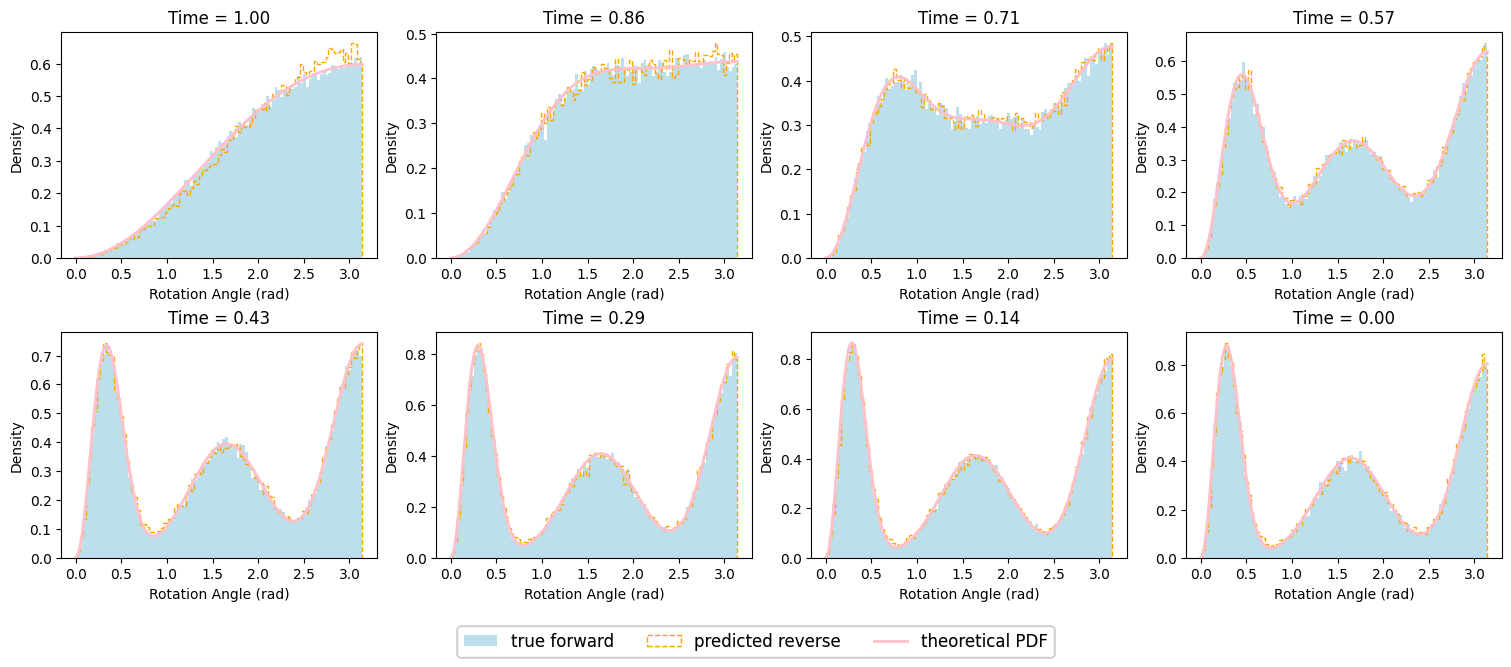
\includegraphics[width=\linewidth]{figures/train_visualization.png}\\
    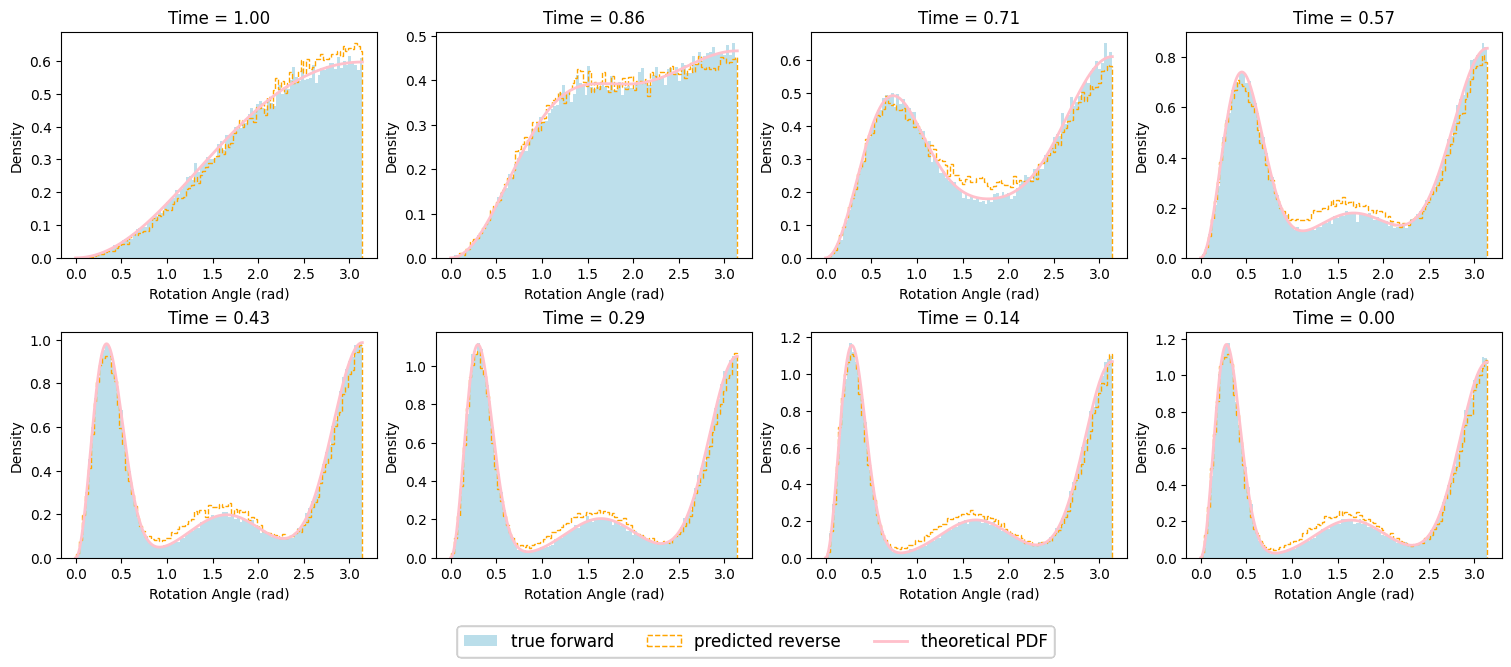
\includegraphics[width=\linewidth]{figures/finetune_visualization.png}
    \caption{Train (top) and fine-tune (bottom) on the marginal densities of the rotation angle $\omega$ for a three-component $\IGSO(3)$ mixture, evaluated at eight evenly spaced noise levels $t\in\qty{1.00,0.86,\dots,0.00}$. The orange dashed lines are the predicted reverse histograms, while the blue shading is the true forward samples. The solid red line is the theoretical PDF given by Proposition~\ref{prop:marginal_igso3}.}
    \label{fig:toy_model_visualization}
\end{figure}

\paragraph{Training the score network.}
The training phase results are depicted in the top panel of Figure~\ref{fig:toy_model_visualization}. This panel shows the learned marginal densities of the rotation angle at eight evenly spaced noise levels during the reverse diffusion process. At the highest noise level ($t=1.00$), the distribution is the uniform Haar measure. As noise decreases, the marginal distributions sharpen, converging towards the true data distribution. The predicted reverse histogram (orange dashed line) accurately matches the true forward samples (blue shading) and theoretical PDF (solid red line) across all time slices, validating the learned score network's accuracy in capturing the $\IGSO(3)$ mixture's true score.

\paragraph{Fine-tuning towards new target values.}
The bottom panel of Figure~\ref{fig:toy_model_visualization} illustrates the marginal rotation angle densities after applying our fine-tuning method (Proposition~\ref{prop:diffusion_model_finetune}) to adjust the mixture component weights to new target values. As the reverse diffusion proceeds, the predicted reverse histograms again closely follow the true forward samples. However, the relative heights of the peaks, corresponding to the mixture component weights, are now shifted according to the target weights $h_i^*$ within minor deviations. This demonstrates that our fine-tuning mechanism effectively reweights the components of the learned distribution to meet specific observable targets without complete retraining, subtly guiding the generative process while preserving the learned structural features.

\subsection{Fine-tuning BioEmu on a small dataset}

Having validated our fine-tuning methodology on the $\SO(3)$ toy model, we now apply it to enhance the BioEmu model for protein folding stability prediction.

\paragraph{Fine-tuning methodology.}
The fine-tuning process leverages a small, curated subset of the MEGAScale dataset, comprising 5 sequences selected to represent a diverse range of experimental $\Delta G$ values from approximately -4.0 kcal/mol to 1.0 kcal/mol, plus one validation sequence. The distribution of folded proportions and $\Delta G$ values for the broader MEGAScale dataset from which these were drawn is shown in Figure~\ref{fig:data_distribution}. In addition to our main fine-tuning idea (Proposition~\ref{prop:kl_divergence_bound}), a series of techniques are employed to improve the fine-tuning stability and computational efficiency (see Proposition~\ref{prop:unbiasedness_loss},~\ref{prop:unbiasedness_gradient},~\ref{prop:rloo},~\ref{prop:time_chunk_aggregation}, and~\ref{prop:inverse_probabilities} for the detailed loss formulation and gradient estimation). The folded proportion $h$ and the folding free energy $\Delta G$ are estimated as described in the Appendix~\ref{sec:folded_proportion_folding_free_energy}. The fine-tuning process is eventually performed on a single NVIDIA H100 GPU with 80 GB memory, using a batch size of 1024 and 20 epochs.

\paragraph{Hyperparameter selection.}
Hyperparameter selection is crucial for the success. Key hyperparameters are detailed in Table~\ref{tab:euler_maruyama_finetune_hyperparameters},~\ref{tab:finetune_hyperparameters},~\ref{tab:folding_stability_hyperparameters} and~\ref{tab:finetune_model_size_hyperparameters}. Hyperparameters for a medium-sized controller model are defined in Table~\ref{tab:finetune_medium_hyperparameters} and~\ref{tab:finetune_model_size_medium_hyperparameters}. Among these, the regularization weight $\lambda$ plays a pivotal role, balancing the adherence to experimental targets against the preservation of the pretrained model's integrity. A small $\lambda$ allows for more aggressive fitting to experimental data but risks distorting the learned distribution (Figure~\ref{fig:finetune_curves_1.0e-06}), while a large $\lambda$ prioritizes fidelity to the pretrained model, potentially limiting adaptation to new target values (Figure~\ref{fig:finetune_curves_1.0e-04}). Through a comprehensive search, an optimal $\lambda = 10^{-5}$ was determined to balance these competing objectives. A medium-sized controller model was also tested, which uses a larger number of hidden layers and hidden dimensions, but the results were not significantly improved (Figure~\ref{fig:finetune_curves_medium}).
\begin{figure}[!ht]
    \centering
    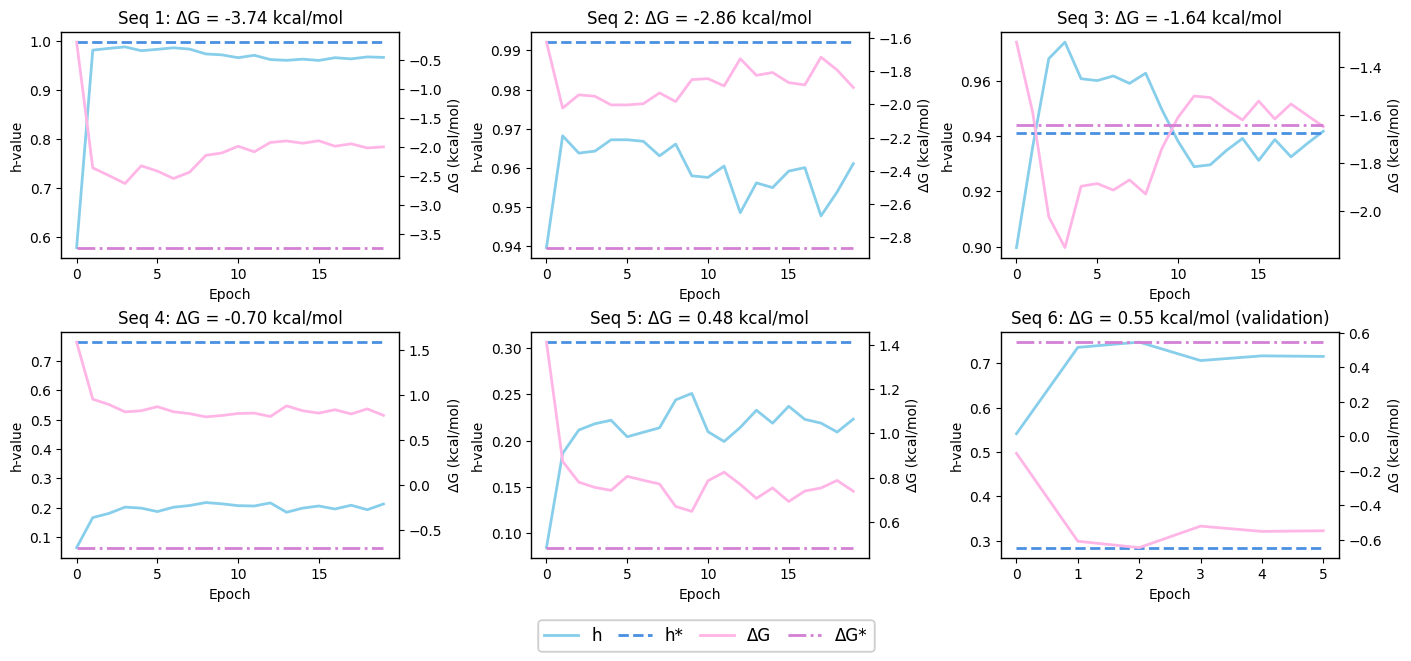
\includegraphics[width=\linewidth]{figures/finetune_h_curves.png}\\
    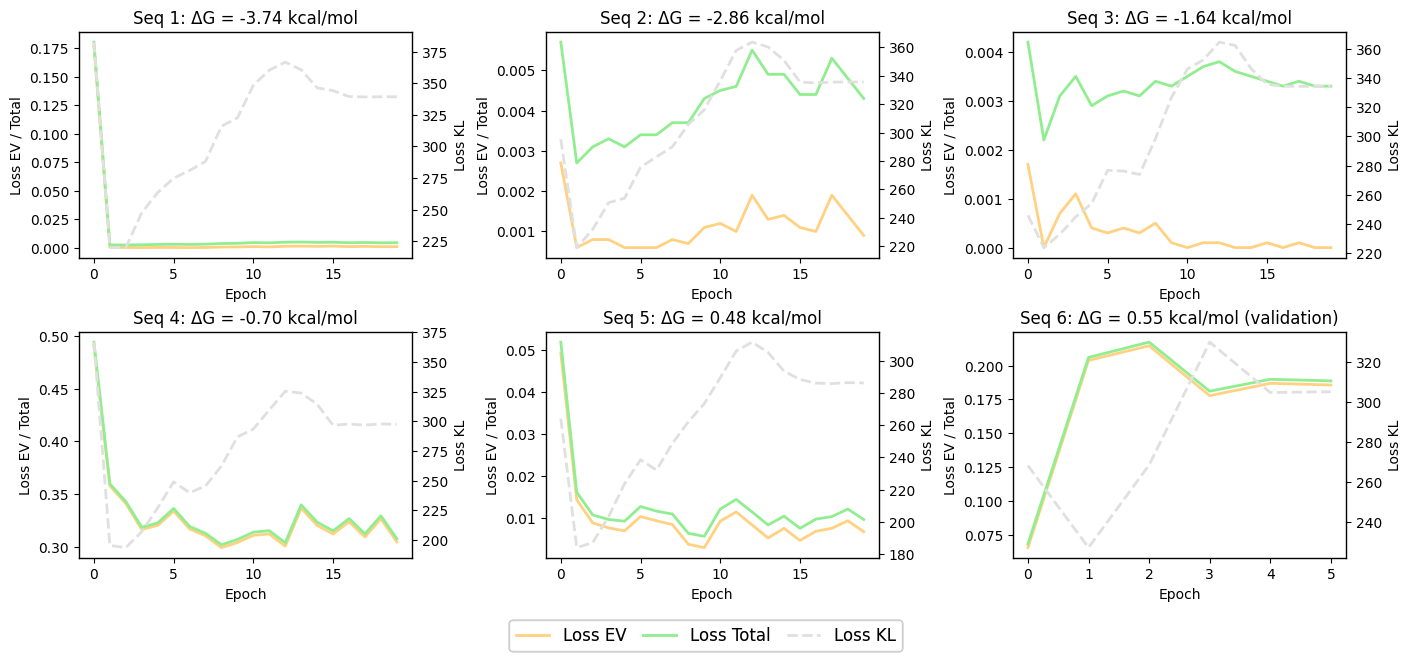
\includegraphics[width=\linewidth]{figures/finetune_loss_curves.png}
    \caption{Fine-tuning performance of BioEmu with optimized hyperparameters. The model was fine-tuned on five randomly selected proteins and evaluated on a single validation sequence. The top panel illustrates the convergence of the expected folded proportion ($h$, blue) and the calculated free energy ($\Delta G$, red) over fine-tuning epochs. The bottom panel displays the evolution of the constituent loss terms: expected value loss (\texttt{loss\_ev}, orange), KL divergence loss (\texttt{loss\_kl}, gray dashed), and total loss (\texttt{loss\_total}, green). Dashed lines in the top panel represent the target observable values.}
    \label{fig:finetune_curves}
\end{figure}

\paragraph{Fine-tuning curves of folded proportion and folding free energy.}
The fine-tuning process, as depicted in Figure~\ref{fig:finetune_curves}, demonstrates successful convergence of predicted folded proportions ($h$) and free energies ($\Delta G$) towards experimental targets for all protein sequences 1 to 5, but not for validation Seq 6, which is not used in the fine-tuning process. In contrast to the decrease in the expected value and total losses, the KL divergence loss initially increases, reflecting an exploration phase, before dropping and settling at a plateau. However, the fine-tuning process encounters challenges with certain sequences. For Seq 4, the model struggles to reach the target $h$ value (around 0.75), with the predicted $h$ plateauing around 0.2. This suggests a difficulty in shifting the model's predictions when the target observable is significantly distant from the initial prediction of the pretrained model. The pretrained BioEmu model embodies a prior over conformational space; if experimental data implies an ensemble drastically different from this prior, the KL divergence penalty resists such large shifts, or the controller may lack the capacity to induce such a change.
Another interesting case is Seq 1. Here, the predicted $h$ value converges very close to its target. Despite this, the predicted $\Delta G$ remains substantially different from the experimental $\Delta G$. This is likely because the conversion of $h$ to $\Delta G$ involves a logarithmic function, which amplifies errors significantly when $h$ is close to 1 (corresponding to very negative $\Delta G$ values).

\paragraph{Visualizing the fine-tuned ensembles.}
Figure~\ref{fig:protein_ensemble} provides a illustrative view of the protein ensembles generated by the fine-tuned BioEmu model for the proteins with the minimum and maximum folding free energy in our set. The root mean square distance (RMSD) of ensembles reflect the targeted stability, with more compact structures for stable proteins and more diverse structures for less stable ones. These visualizations help confirm that the fine-tuning process leads to structurally meaningful changes in the generated ensembles, consistent with the targeted stability.

\begin{figure}[!ht]
    \centering
    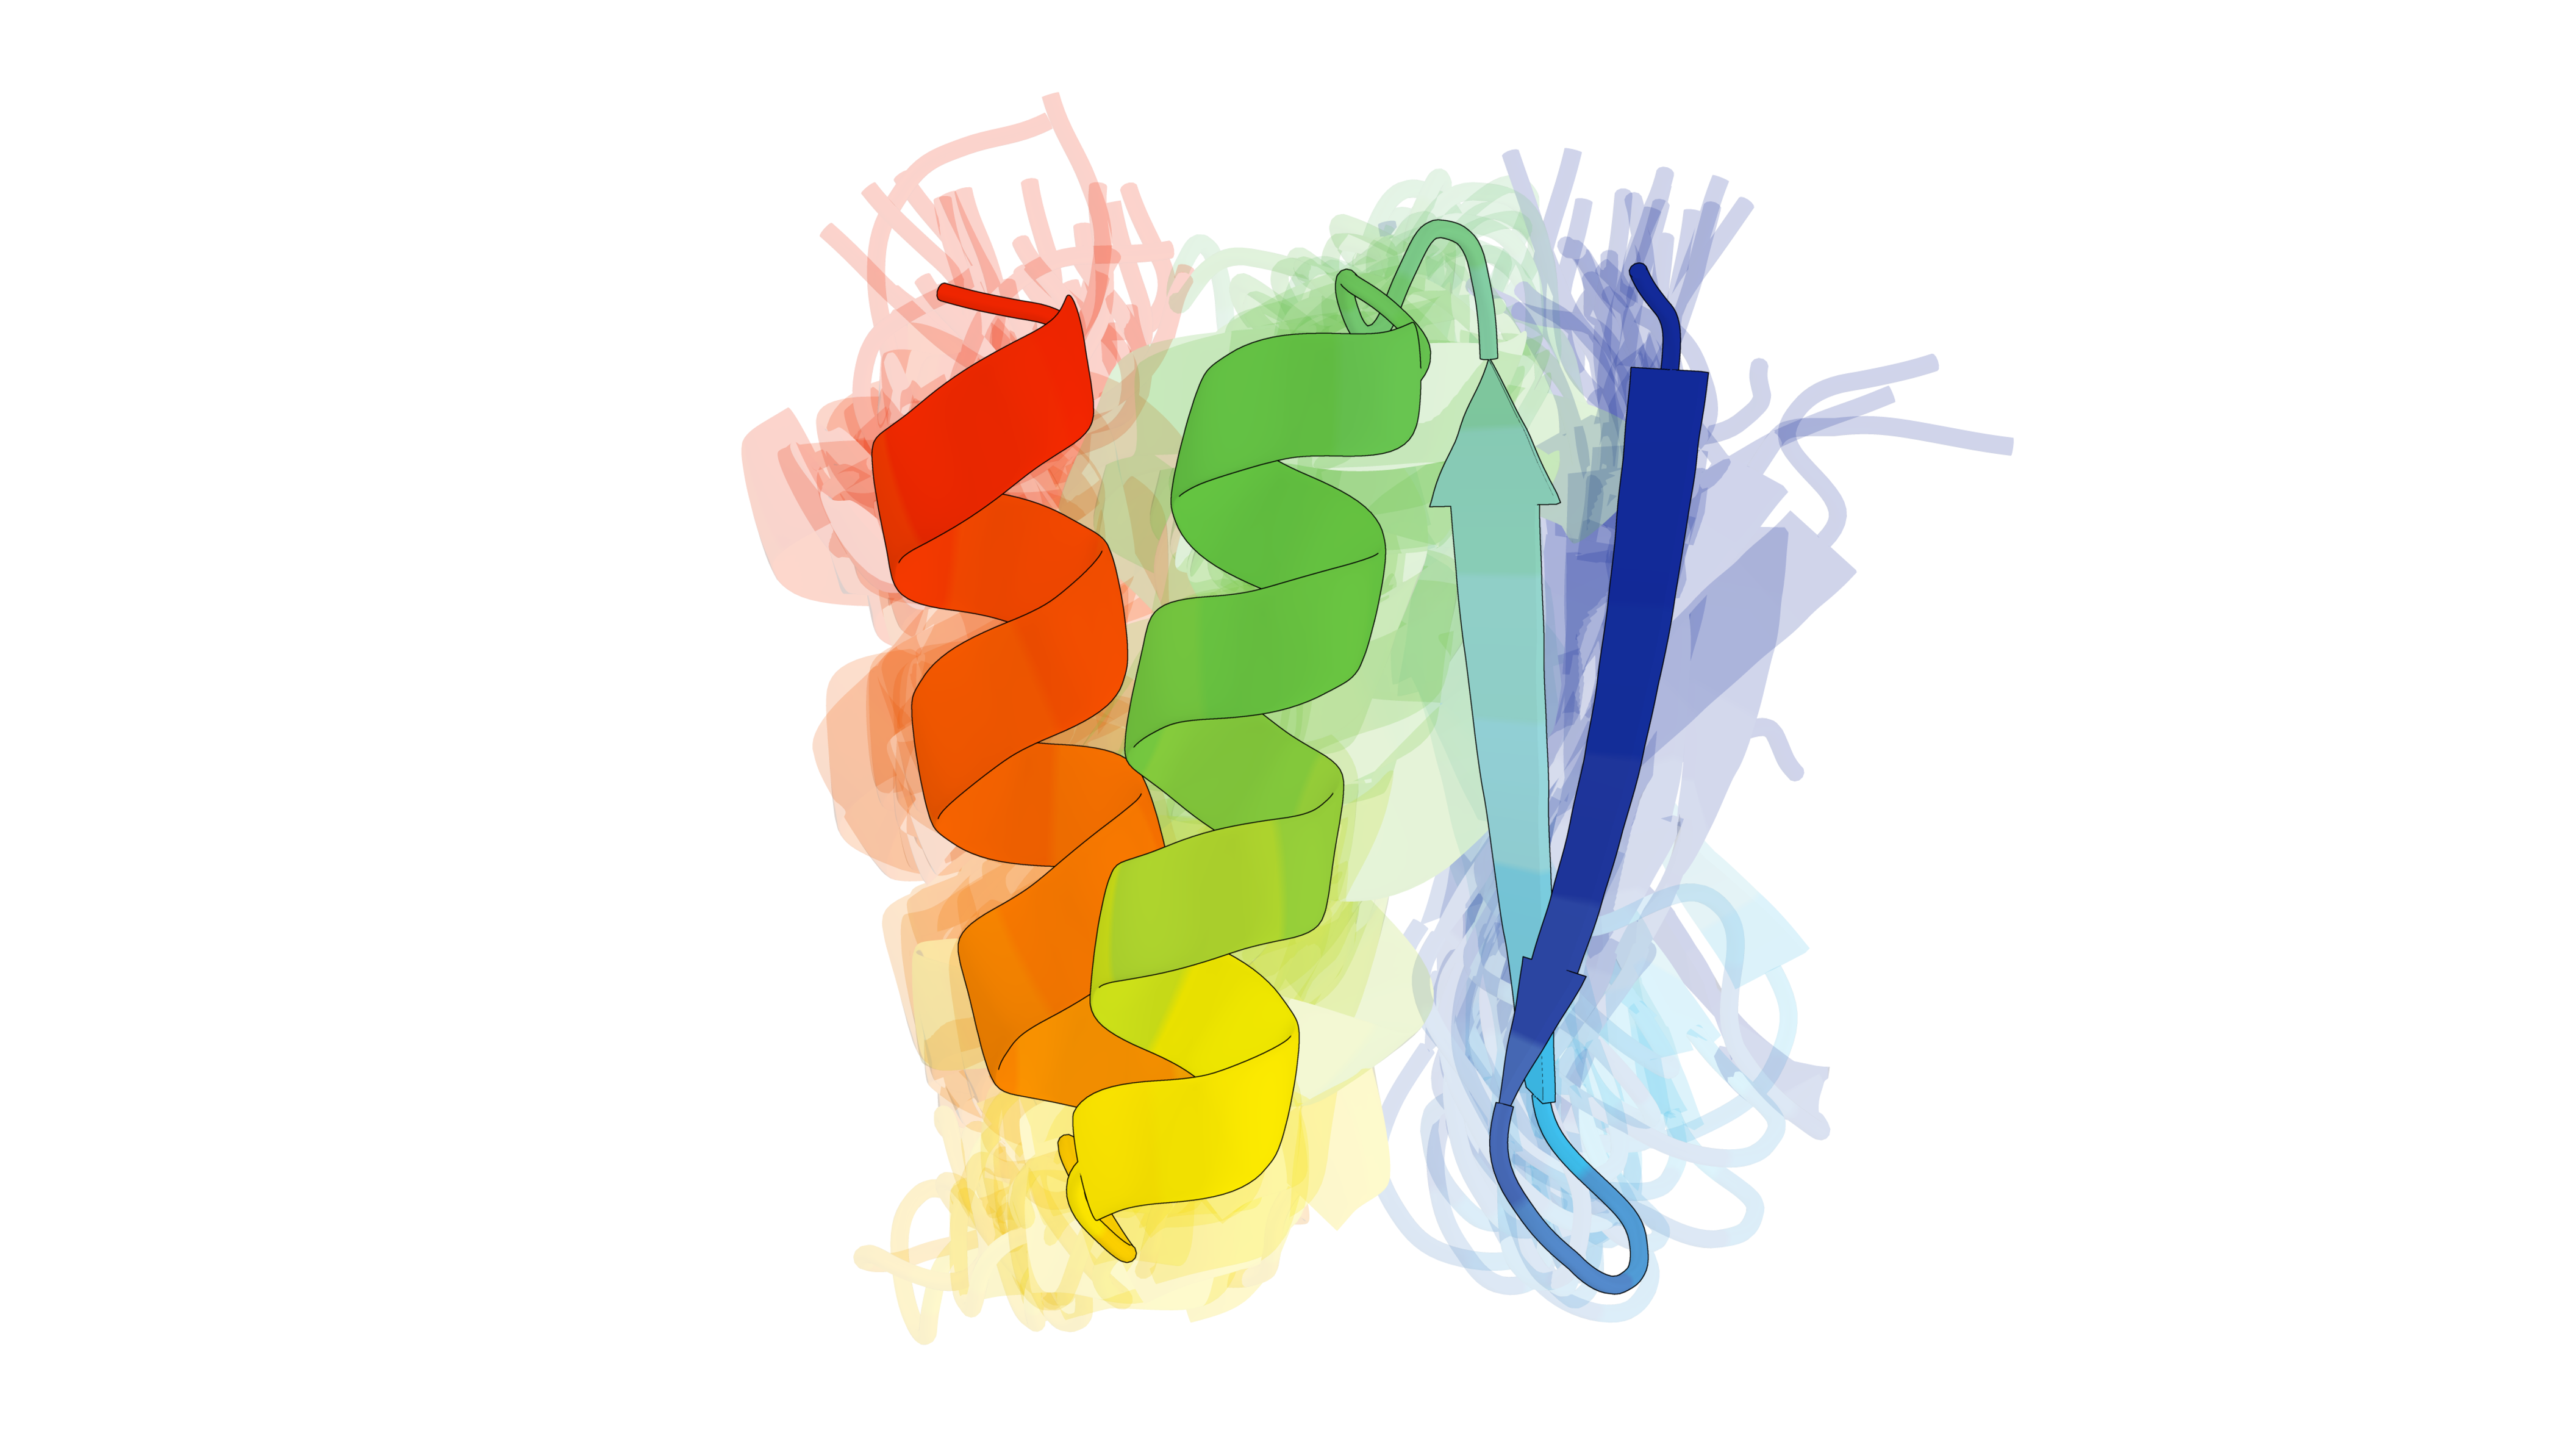
\includegraphics[width=0.45\linewidth]{figures/min.png}
    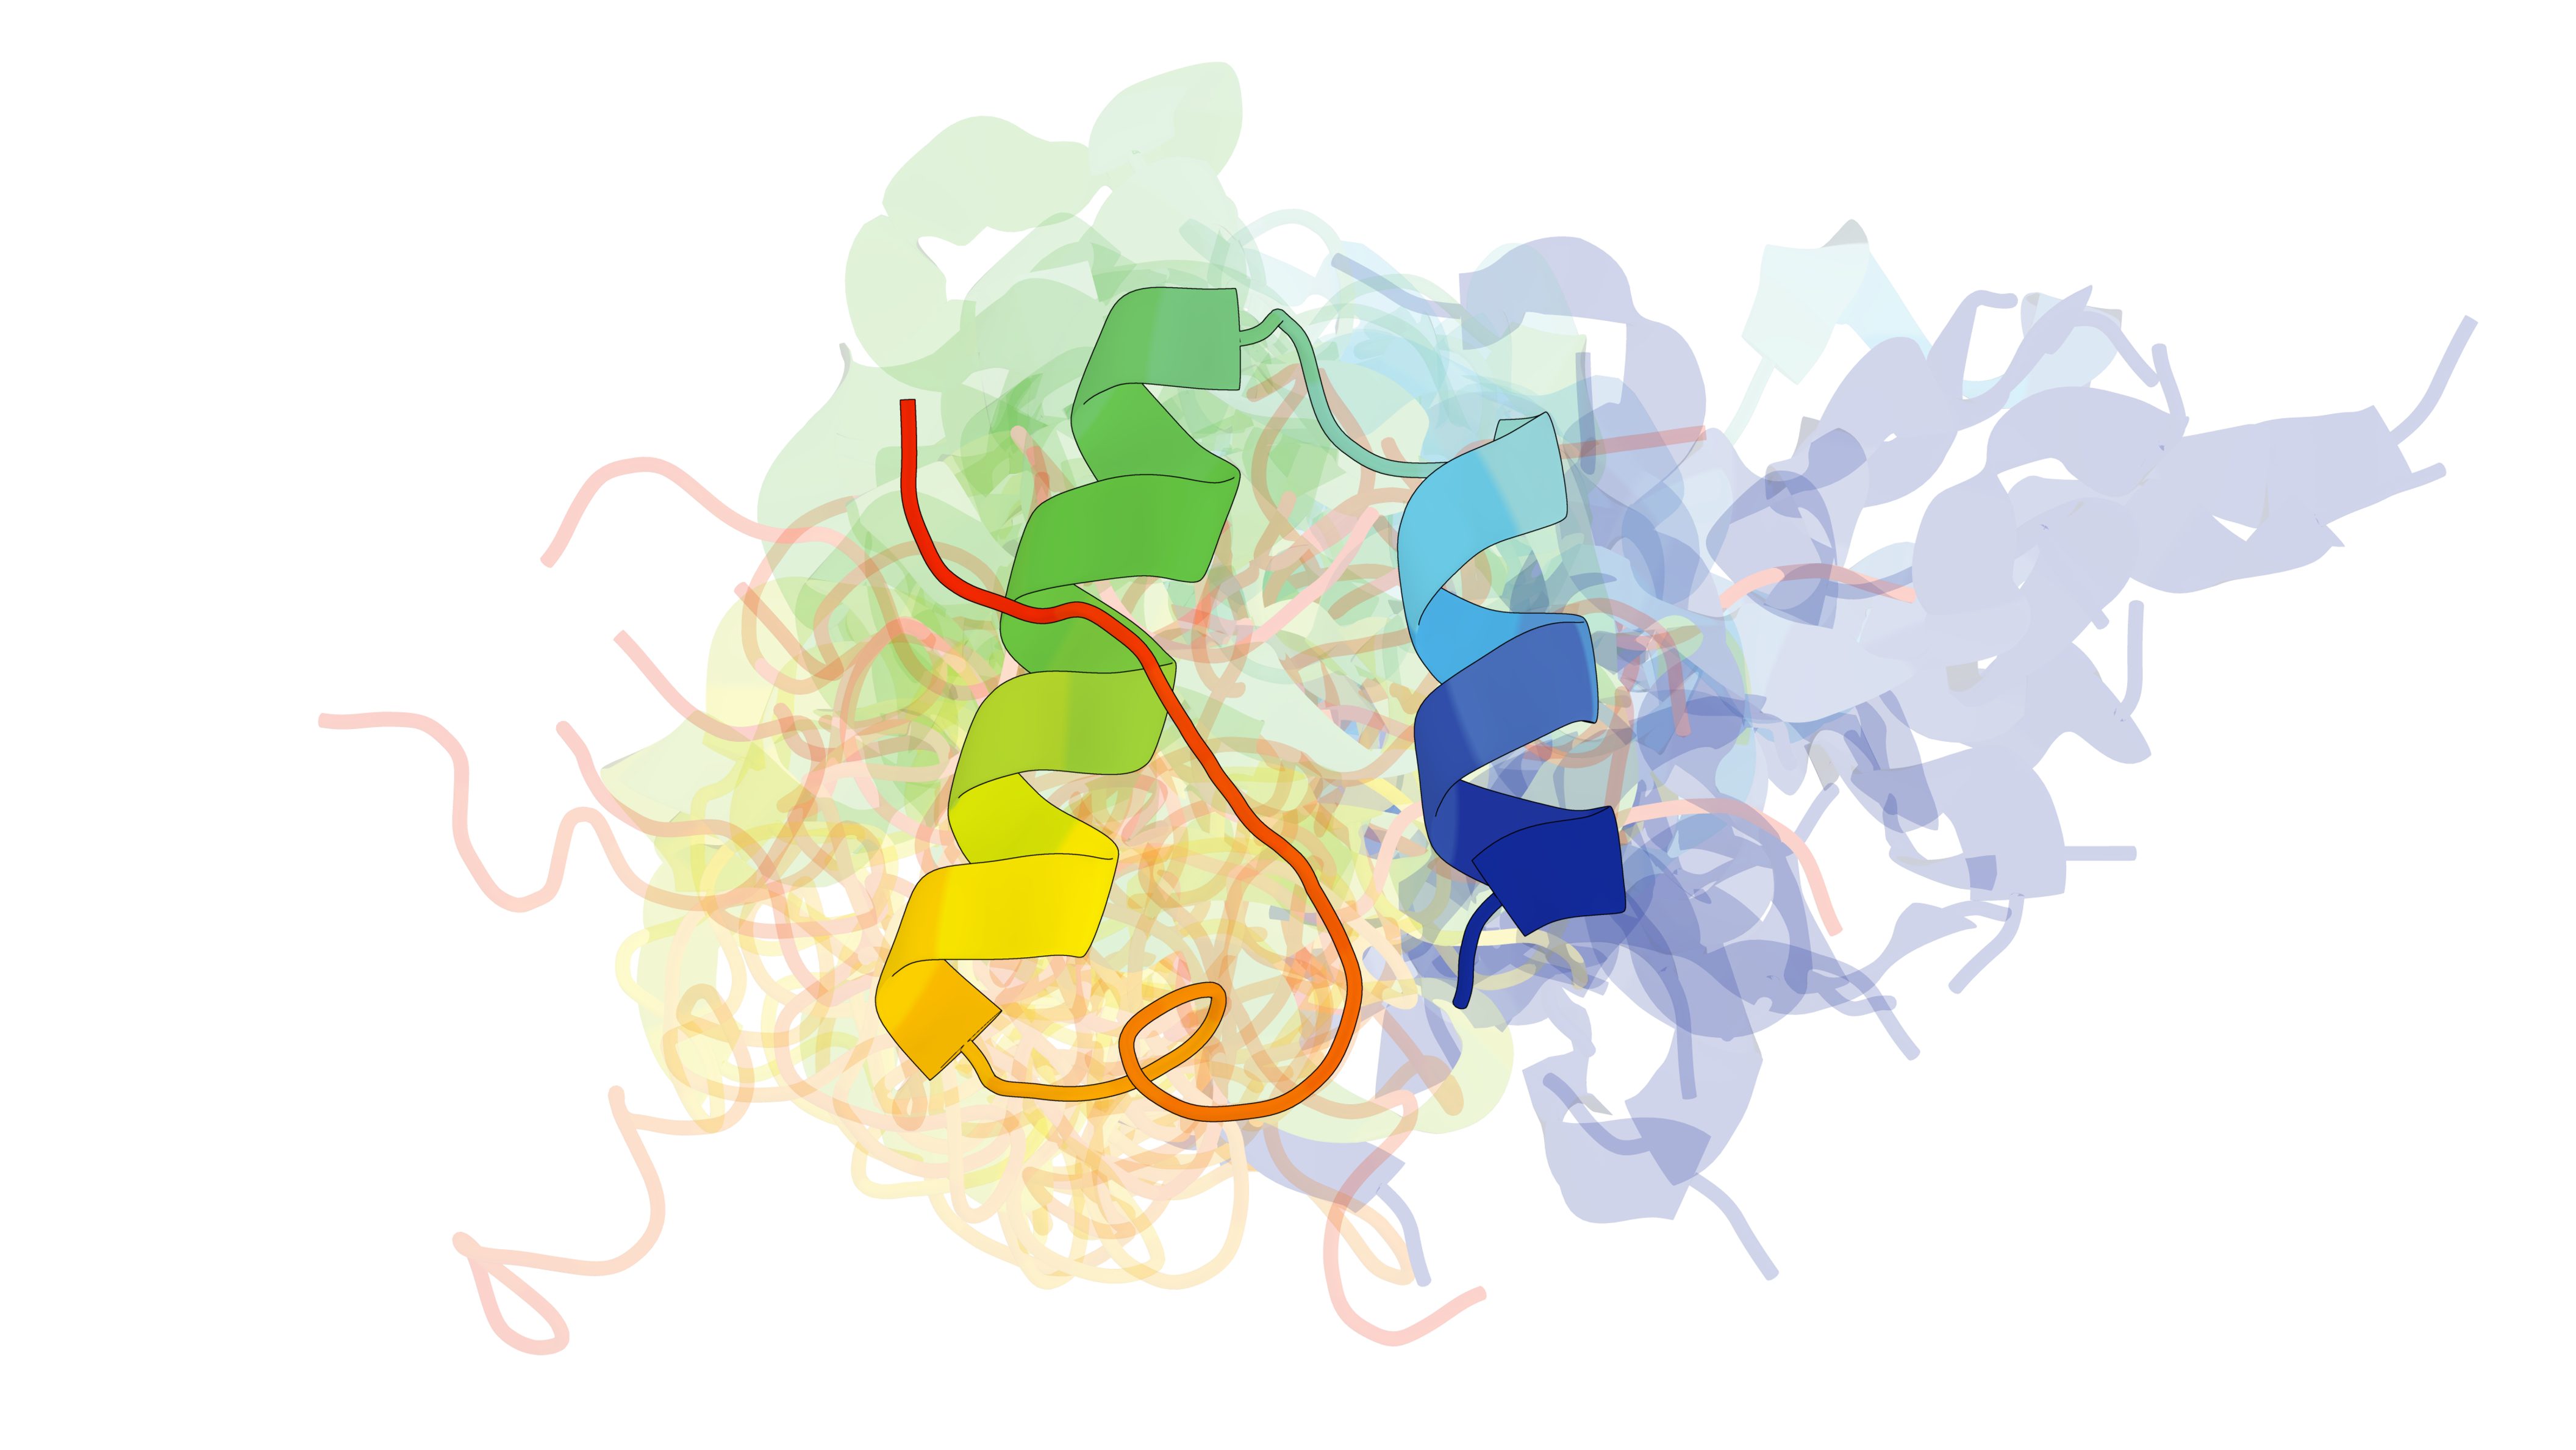
\includegraphics[width=0.45\linewidth]{figures/max.png}\\
    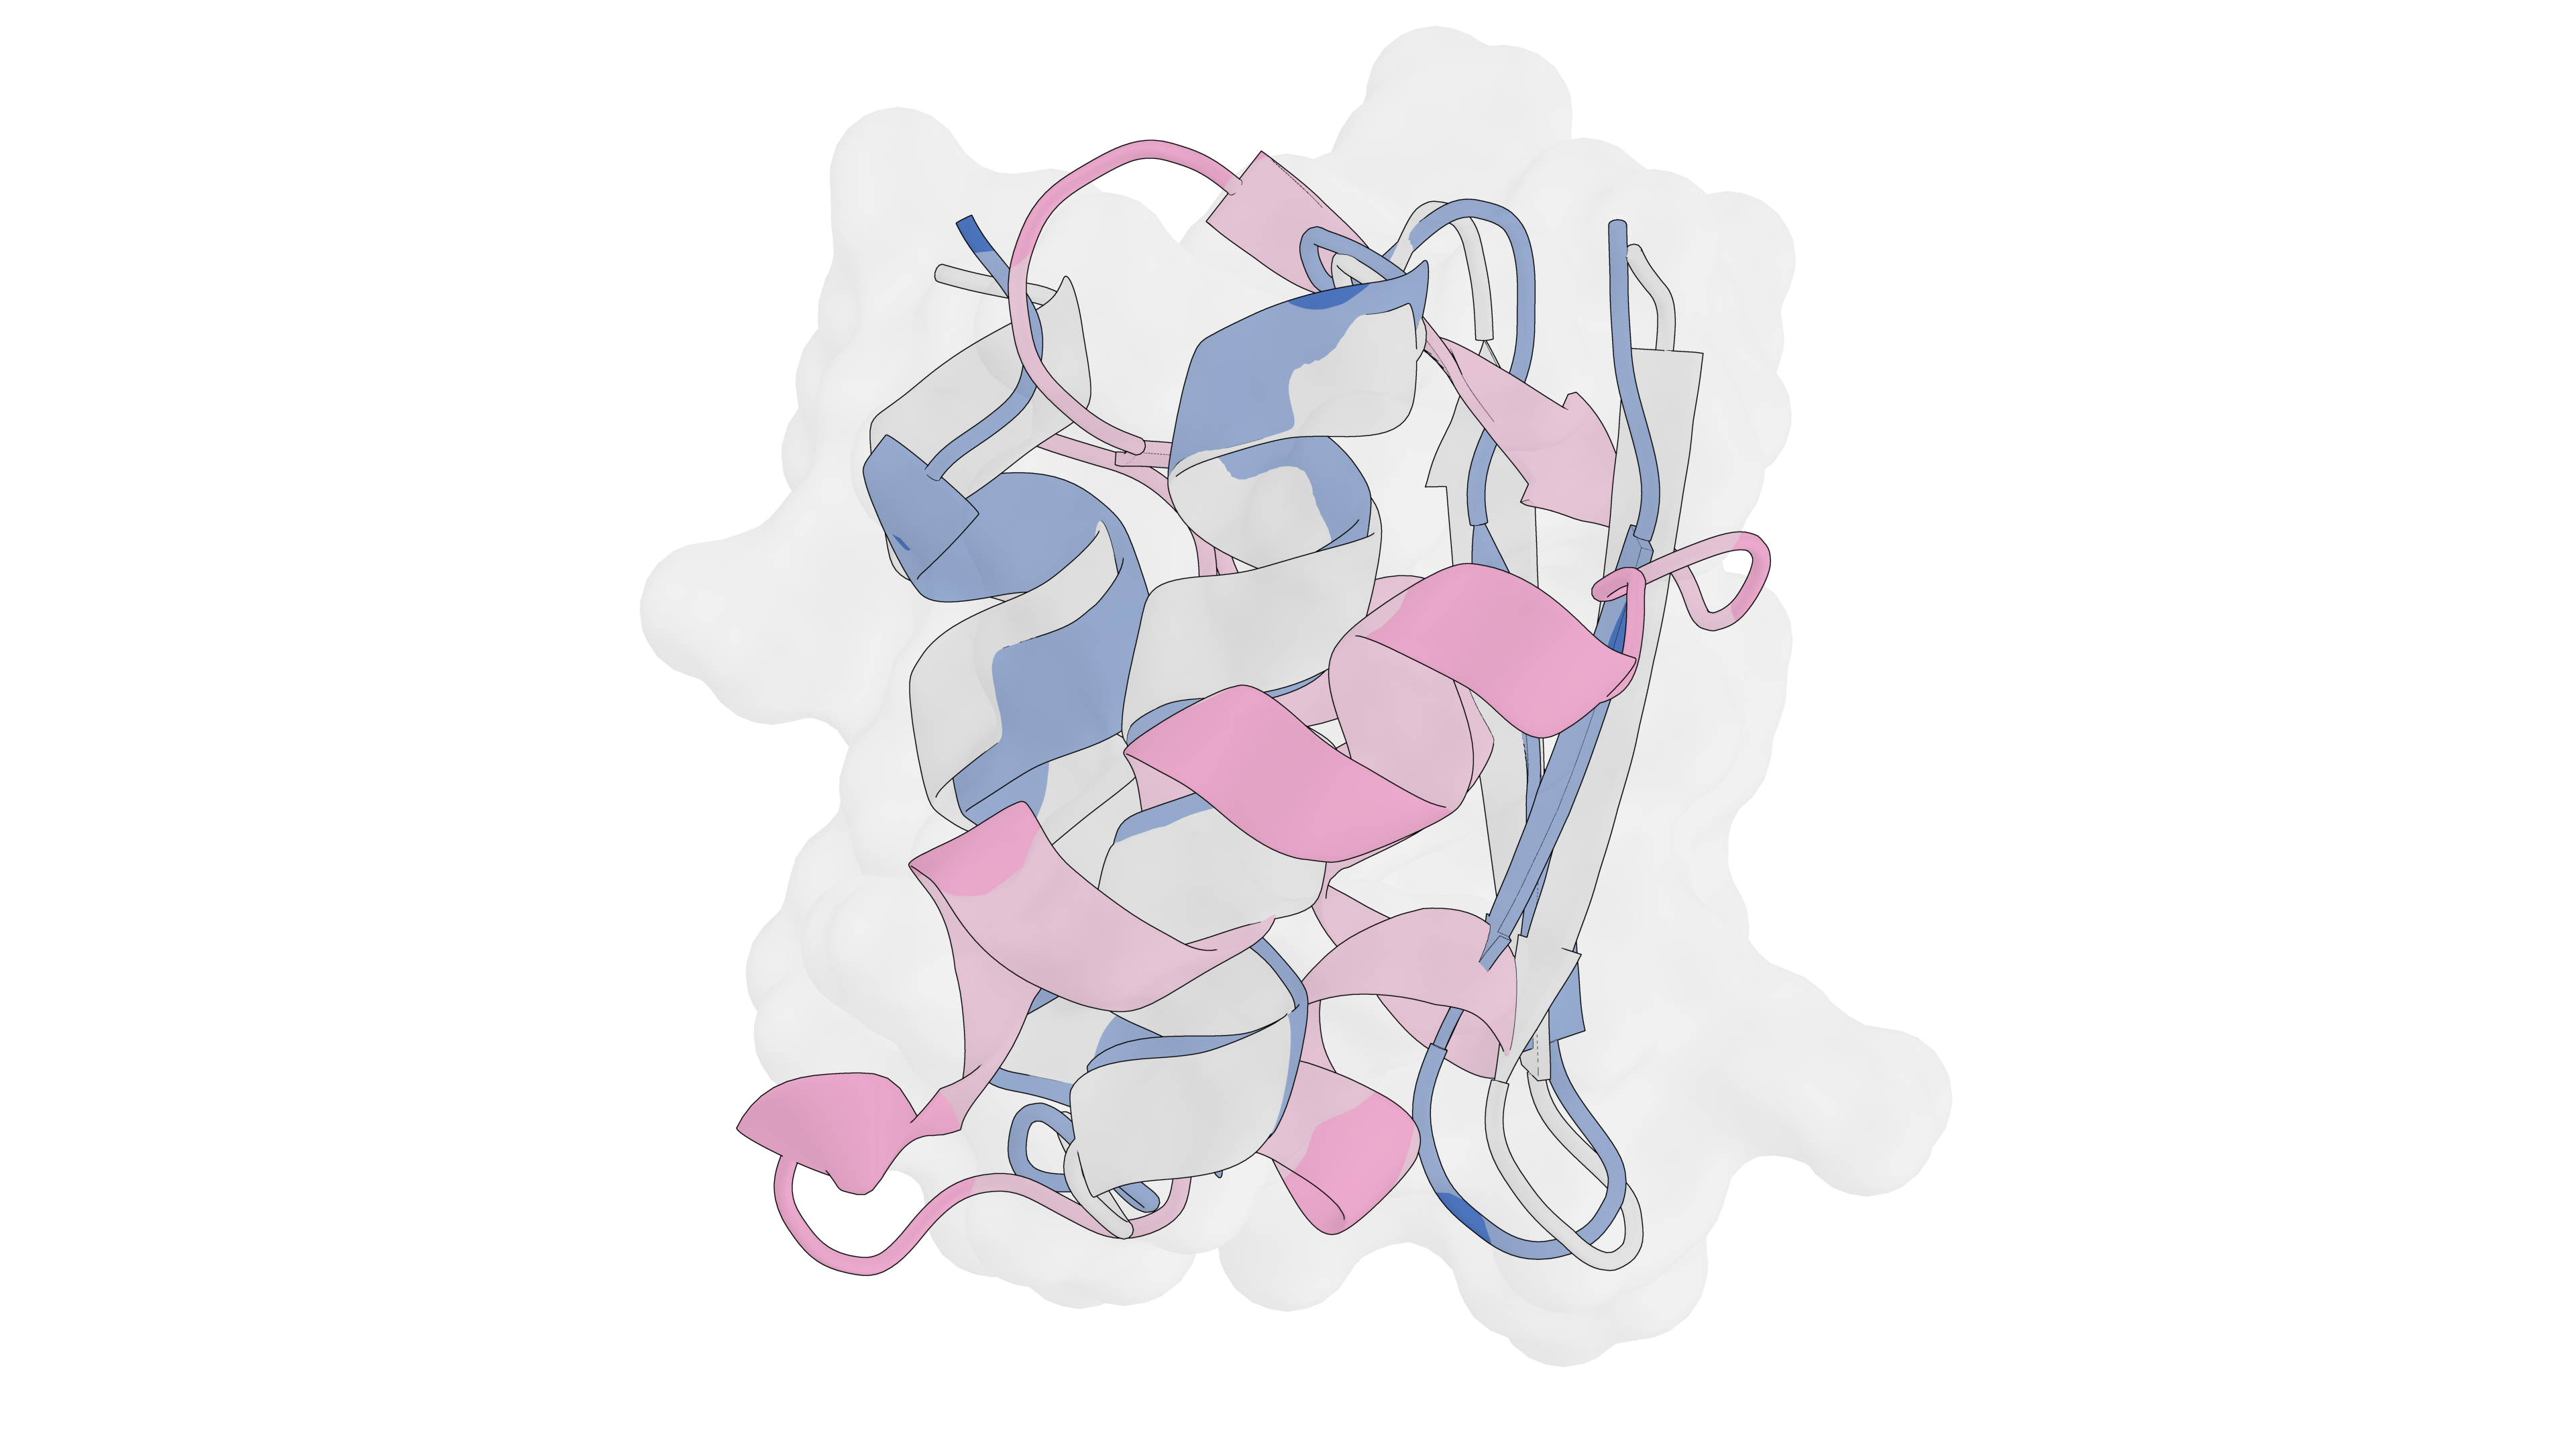
\includegraphics[width=0.45\linewidth]{figures/min_compare.png}
    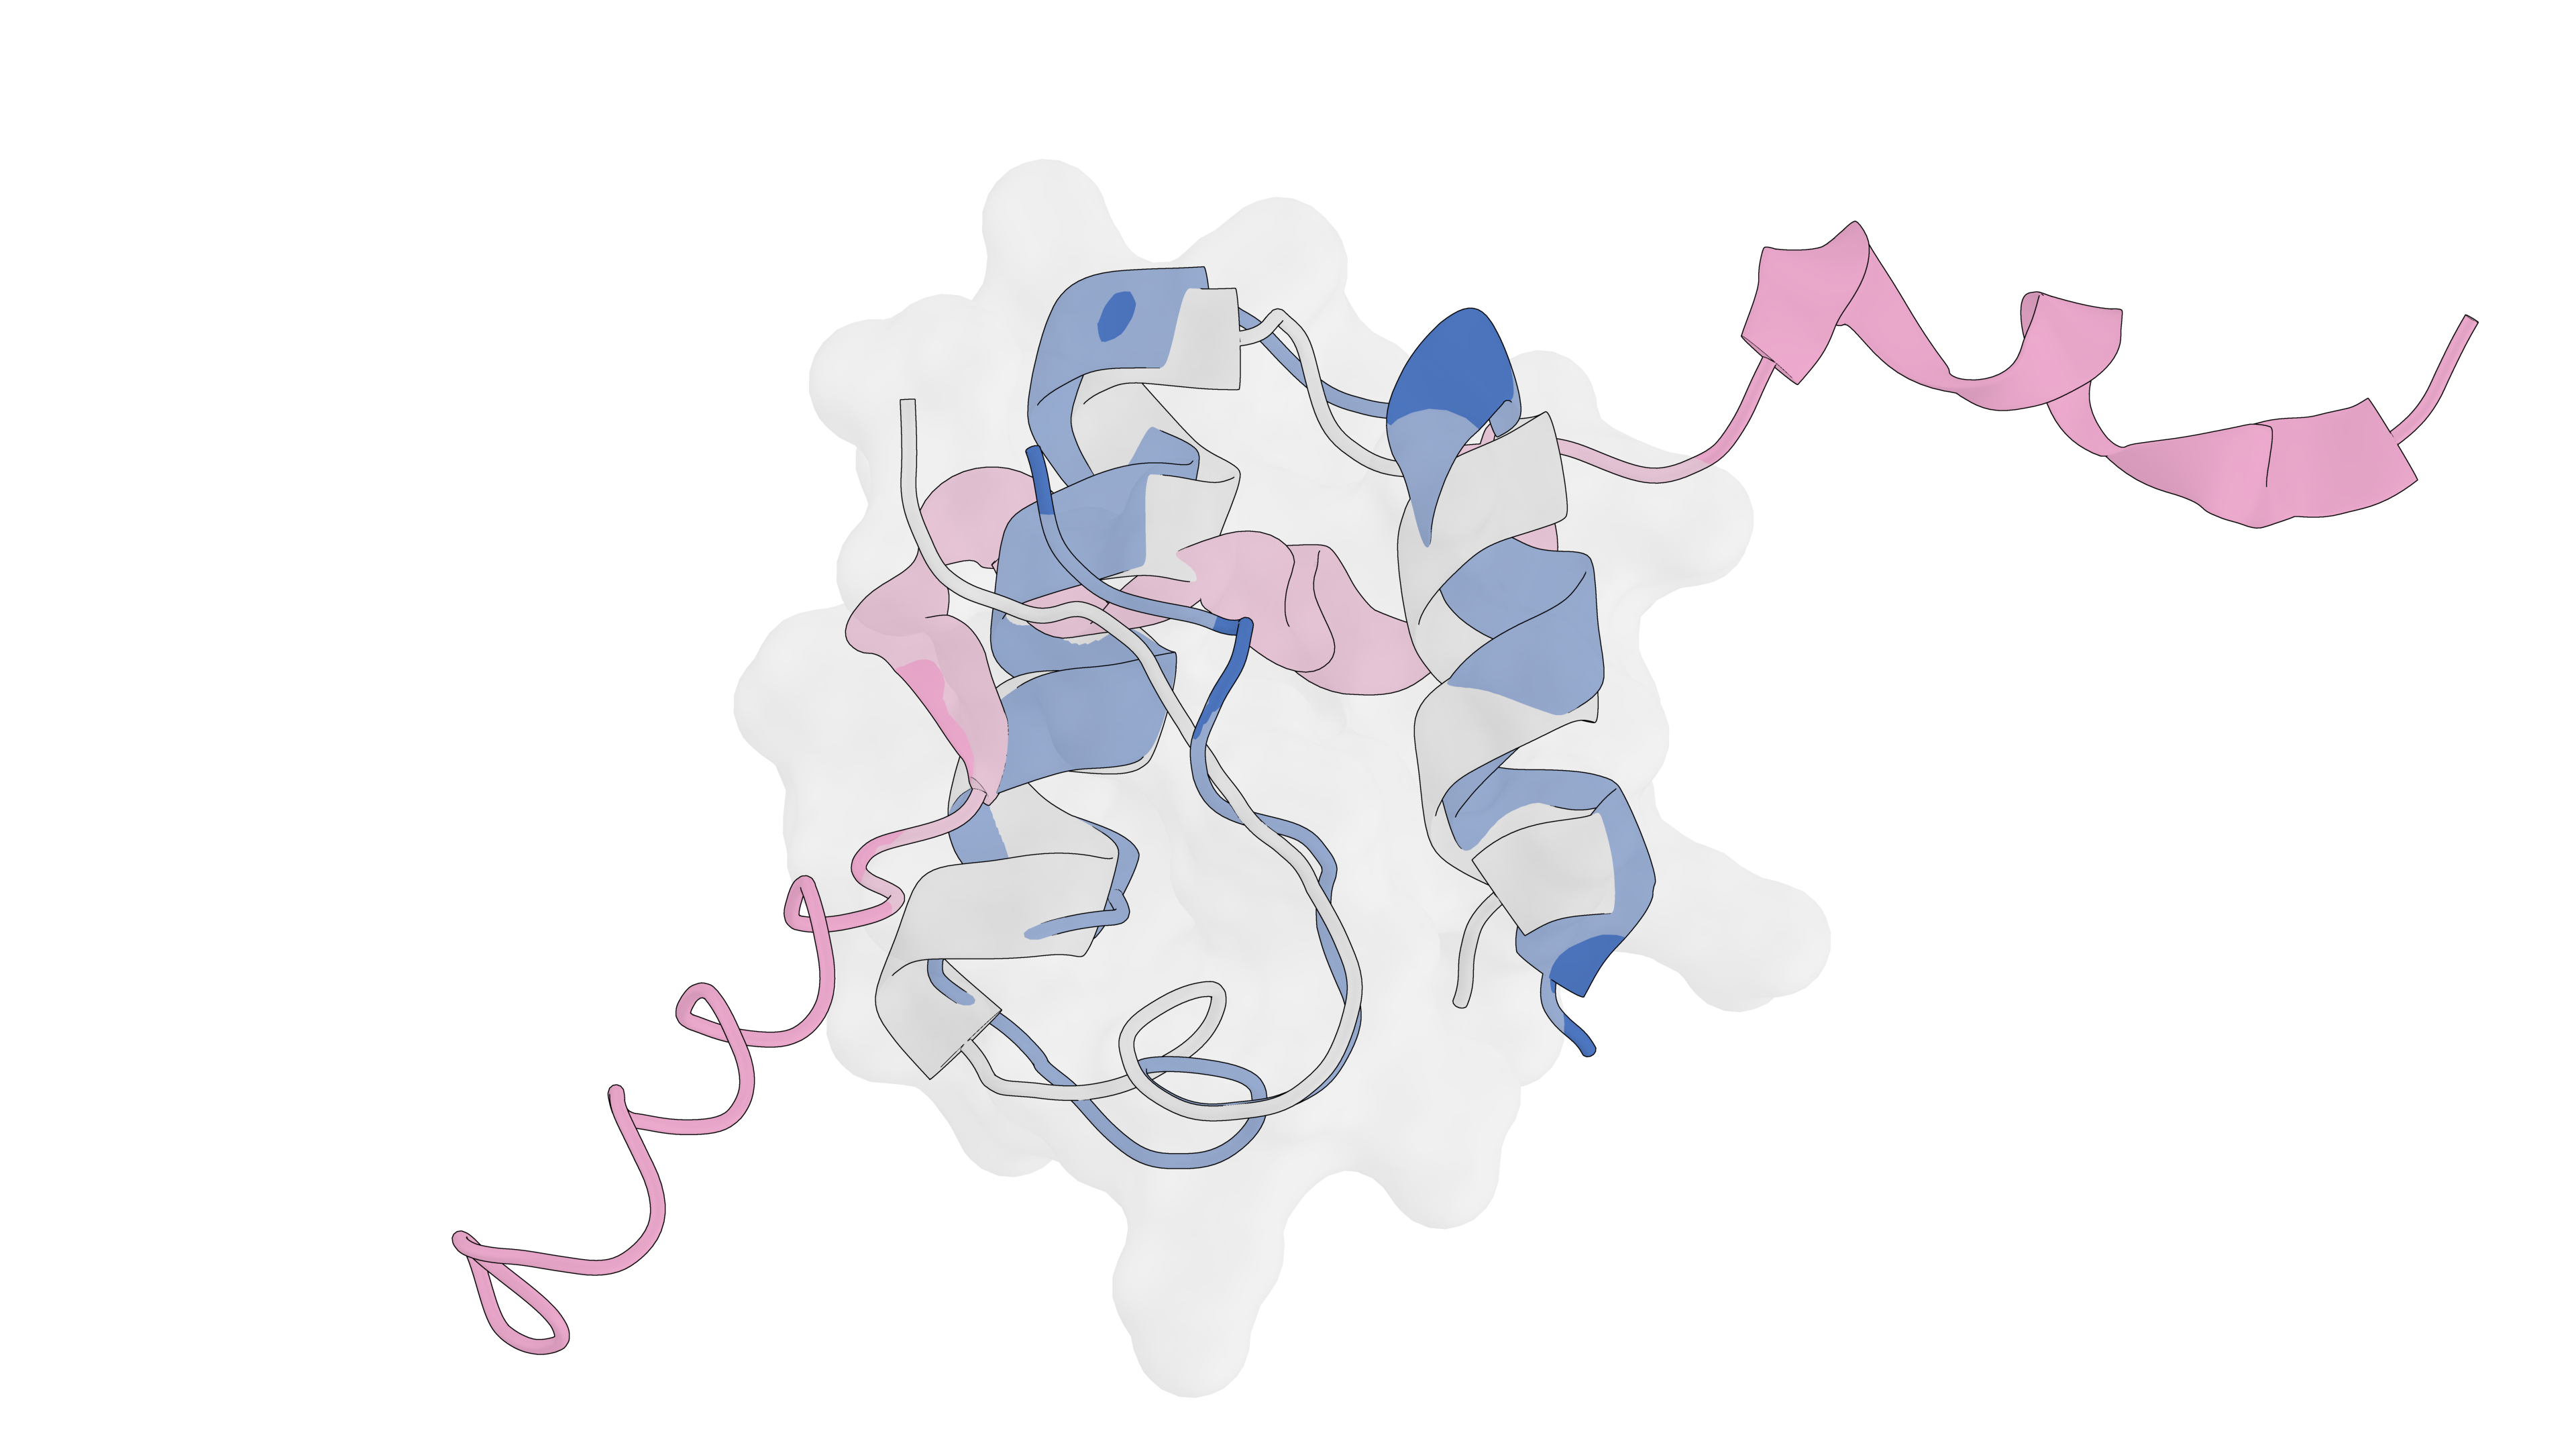
\includegraphics[width=0.45\linewidth]{figures/max_compare.png}
    \caption{Visual illustration of the protein ensemble after fine-tuning for the two proteins with the smallest (left) and largest (right) $\Delta G$ values. The top row shows all the generated conformations (transparent) and the reference conformation (opaque) for each protein. The bottom row highlights the most native-like (blue, lowest RMSD) and most deviated (red, highest RMSD) structures. The reference conformation is colored in gray.}
    \label{fig:protein_ensemble}
\end{figure}

\paragraph{Distributional shifts of key observables.}
The impact of fine-tuning on the distributions of key observables is quantified in Figure~\ref{fig:metrics_distribution}. For the ``min'' protein (highly stable), which initially shows a single peak in these three distributions, fine-tuning shifts the distributions towards a certain direction that indicates a more diverse conformational ensemble. Conversely, for the ``max'' protein, which is initially less stable and often characterized by a bimodal distribution representing folded and unfolded states, fine-tuning acts by reweighting the proportions of these existing conformations. This process typically aims to increase the population of the folded state, thereby making the protein appear more stable, while preserving the essential bimodal character of the conformational landscape. These distributional shifts provide compelling evidence that the fine-tuning process is not merely matching a single expected value but is genuinely reshaping the probability landscape of the generated conformational ensembles in a manner consistent with the target experimental stabilities by modulating the balance between pre-existing states.

\begin{figure}[!ht]
    \centering
    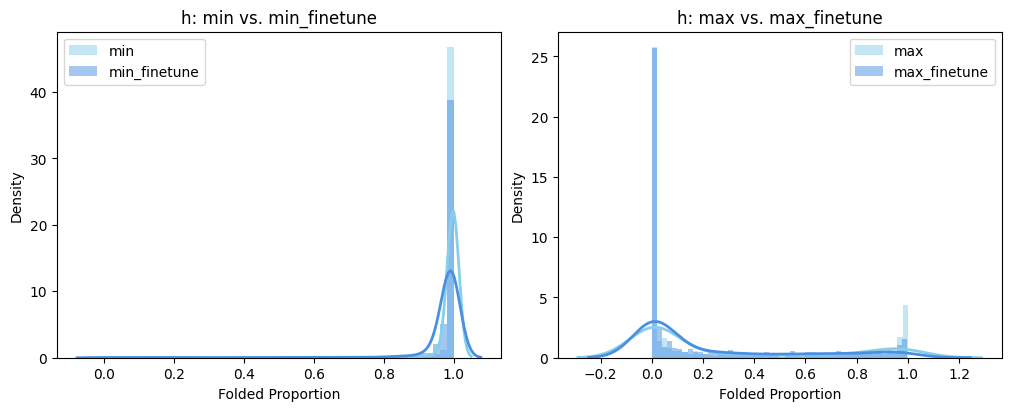
\includegraphics[width=\linewidth]{figures/h_distribution.png}\\
    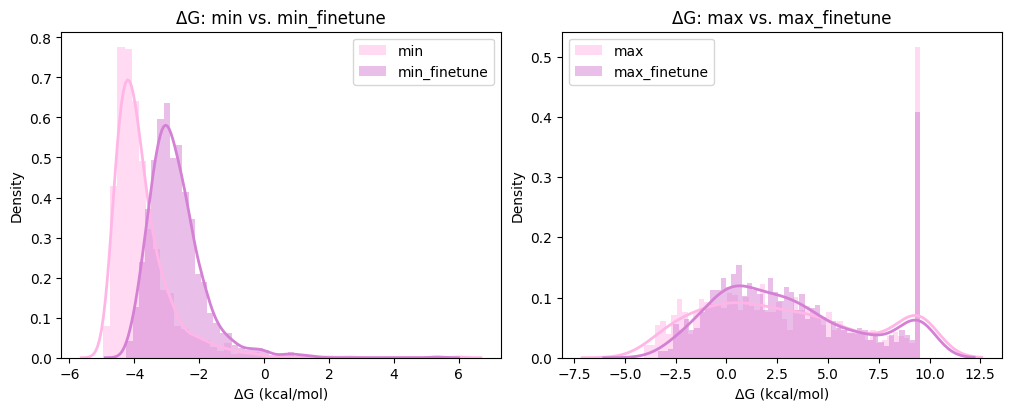
\includegraphics[width=\linewidth]{figures/dG_distribution.png}\\
    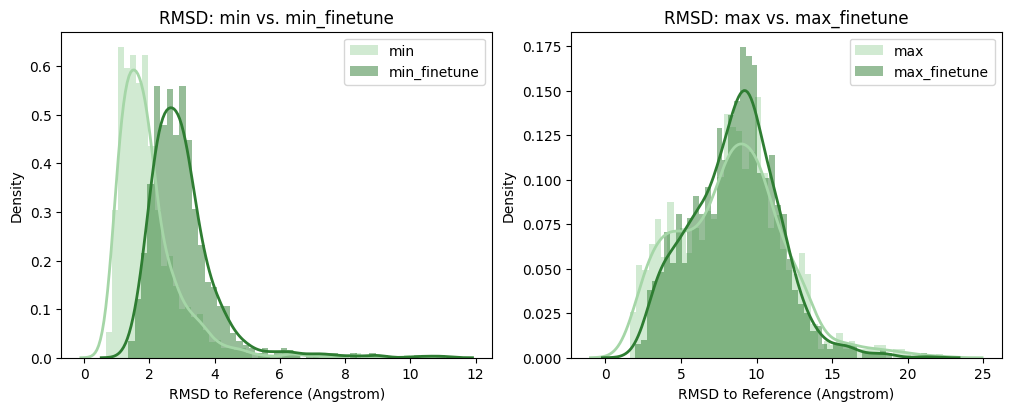
\includegraphics[width=\linewidth]{figures/rmsd_distribution.png}
    \caption{Distributions of three relevant observables $h$ (folded proportion, top, blue), $\Delta G$ (folding free energy, middle, red), and RMSD (bottom, green) for 2 of the 5 proteins with the smallest (named ``min'') and largest (named ``max'') $\Delta G$ values. Light colors show the original BioEmu distribution, while dark colors show the fine-tuned distribution.}
    \label{fig:metrics_distribution}
\end{figure}

\paragraph{Correlation between experimental and predicted $\Delta G$ values.}
Figure~\ref{fig:correlation} assesses the predictive accuracy of the fine-tuned model by plotting experimental $\Delta G$ values against the $\Delta G$ values predicted from the fine-tuned ensembles, using both root mean square distance between distance matrices (dRMSD)-based (left panel) and the fraction of native contacts (FNC)-based (right panel) estimation methods. The points generally cluster around the y=x line (dashed line), indicating a good correlation between experimental and predicted values.

\begin{figure}[!ht]
    \centering
    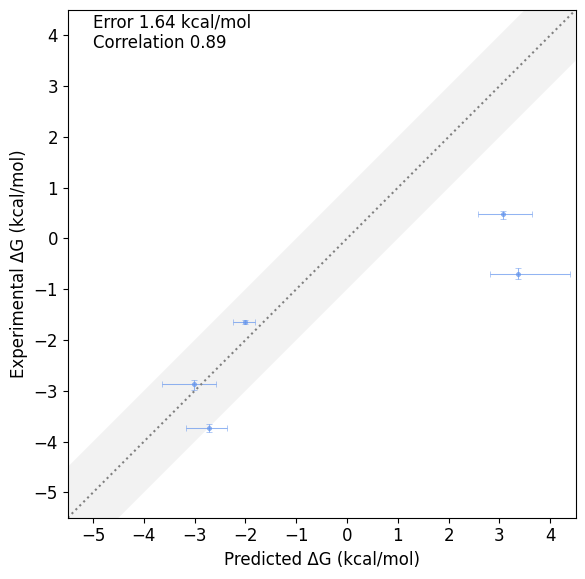
\includegraphics[width=0.45\linewidth]{figures/correlation_dRMSD.png}
    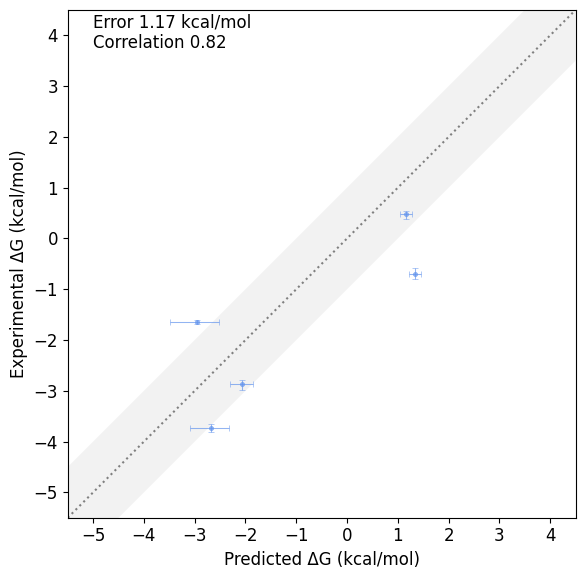
\includegraphics[width=0.45\linewidth]{figures/correlation.png}
    \caption{Correlation between the experimental $\Delta G$ values and the predicted $\Delta G$ values with two different estimation methods (dRMSD, left; and FNC, right) for the 5 proteins used for fine-tuning. The dashed line shows the $y=x$ line. Error bars and the shaded area show the 97.5\% confidence interval of the correlation coefficient.}
    \label{fig:correlation}
\end{figure}

\paragraph{Comparison of different observable estimation methods.}
The consistency of different observable estimation methods is explored in Figure~\ref{fig:dRMSD_vs_FNC}. This figure compares the folded proportion (left panel) and folding free energy (right panel) estimated using the dRMSD-based approach versus the FNC-based approach. For folded proportion, there is almost no clear correlation between the two estimators, although the marginal distribution of each looks similar. For folding free energy, a correlation is discernible, but it appears biased and curved. While there can be good correlation for slightly negative $\Delta G$ values, the relationship exhibits largely different slopes across the range. Discrepancies between estimators could indicate sensitivities in how ``foldedness'' are defined and quantified. This suggests that while the current naive estimation functions are serviceable, there is potential for improvement, perhaps by using more sophisticated, or even trainable, models for these observables, which could alleviate issues like the one observed for Seq 1.

\begin{figure}[!ht]
    \centering
    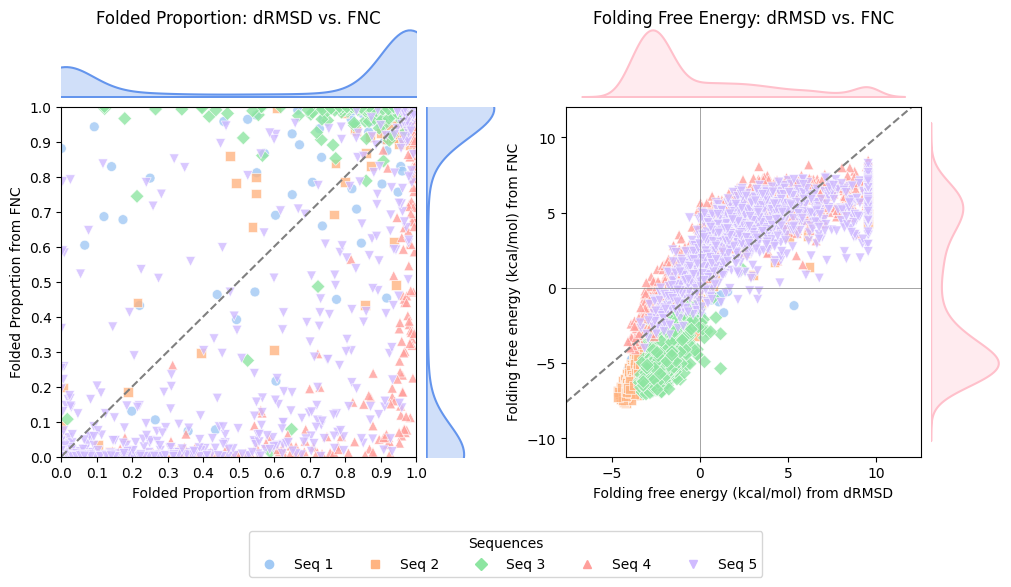
\includegraphics[width=\linewidth]{figures/dRMSD_vs_FNC.png}
    \caption{Correlation between the folded proportion (left) and the folding free energy (right) for the 5 proteins used for fine-tuning with the two different estimation methods (dRMSD, $x$-axis; and FNC, $y$-axis). The dashed line shows the $y=x$ line, and histograms on the top and right show the distribution of the values for each method.}
    \label{fig:dRMSD_vs_FNC}
\end{figure}

\section{Discussion}

Our work introduces a novel fine-tuning approach for diffusion models on $\SE(3)$, specifically targeting the prediction of protein folding stability. The main findings, challenges, and potential avenues for future work are discussed below.

\subsection{Main findings}

The fine-tuning methodology was first validated on a synthetic $\IGSO(3)$ mixture model. As shown in Figure~\ref{fig:toy_model_visualization}, the method successfully learned and then adjusted the mixture component weights to match new target values, confirming the correctness of the underlying mathematical framework (Proposition~\ref{prop:marginal_igso3},~\ref{prop:stein_score},~\ref{prop:diffusion_model_finetune}) on this non-Euclidean manifold. This provides a strong foundation for its application to the more complex $\SE(3)$ manifold of protein structures.

When applied to fine-tune BioEmu on a subset of the MEGAScale dataset, our approach demonstrated its capability to improve predictions for several protein sequences. As seen in Figure~\ref{fig:finetune_curves}, for sequences with moderate target $\Delta G$ values (e.g., Seq 2, 3, 5), the predicted folded proportion $h$ and subsequently the calculated $\Delta G$ converged towards their experimental targets. This suggests an improvement over the original BioEmu predictions for these specific cases by incorporating experimental data. The fine-tuned model was also able to generate meaningful and diverse conformational ensembles (Figures~\ref{fig:protein_ensemble} and~\ref{fig:metrics_distribution}), indicating that the fine-tuning process reshapes the probability landscape in a structurally relevant manner.

A significant practical advantage of our method is its computational efficiency. The fine-tuning process, utilizing a batch size of 1024 samples and 200 diffusion steps per sample, can be performed on a single NVIDIA H100 GPU with 80GB of memory. This efficiency is largely due to the use of a small controller term and the time-chunk aggregation method for gradient estimation (Proposition~\ref{prop:time_chunk_aggregation}), which avoids backpropagation through the entire, potentially very long, diffusion trajectory.

The current naive functions for estimating folded proportion $h$ from dRMSD and FNC (Appendix~\ref{sec:folded_proportion_folding_free_energy}) proved serviceable. However, as Figure~\ref{fig:dRMSD_vs_FNC} illustrates, there are discrepancies between these estimators, particularly for folding free energy. This suggests that while the fine-tuning mechanism itself works, the accuracy of the final $\Delta G$ prediction is sensitive to the choice and fidelity of these observable functions. Future work could explore trainable or more sophisticated biophysical models for these observables.

\subsection{Major challenges}

Despite the successes, two main challenges were identified. First, the model struggled to fine-tune effectively when the target observable value $h^*$ was very distant from the pretrained model's initial prediction. This was evident for Seq 4 (Figure~\ref{fig:finetune_curves}), where the predicted $h$ plateaued far from the target. This limitation might stem from the KL divergence term in the loss function (Proposition~\ref{prop:kl_divergence_bound}), which penalizes large deviations from the pretrained distribution, or it could indicate that the controller network lacks the capacity to induce such substantial shifts.

Second, for proteins with very high stability (e.g., Seq 1, where $h^*$ is close to 1, corresponding to a very negative $\Delta G^*$), achieving a close match for $h$ did not always translate to an accurate $\Delta G$ prediction (Figure~\ref{fig:finetune_curves}). The logarithmic relationship between $h$ and $\Delta G$ means that small errors in $h$ when $h \approx 1$ can lead to large errors in $\Delta G$. An alternative approach could be to directly minimize the discrepancy in the free energy space. For instance, one could define the loss as $(-RT\log(\mathbb{E}[h]/(1-\mathbb{E}[h])) - \Delta G^*)^2$, where $R$ is the gas constant and $T$ is the temperature. The unbiased gradient estimation techniques developed in this work (e.g., Proposition~\ref{prop:unbiasedness_gradient},~\ref{prop:diffusion_model_finetune}) could potentially be adapted to optimize such an objective, which might mitigate the sensitivity observed for highly stable proteins.

\subsection{Minor issues and future directions}

Several smaller issues and areas for improvement were noted. The current implementation relies on the Euler-Maruyama SDE solver (Algorithm~\ref{alg:em_predictor_so3}) because the Girsanov theorem-based controller (Proposition~\ref{prop:diffusion_model_finetune},~\cite{girsanov_on_manifolds, girsanov_in_riemannian}) requires access to the Wiener increments $\dd \mathbf{W}_t^\mathcal{M}$. This precludes the straightforward use of more advanced ODE-based denoisers~\cite{dpmsolver} or higher-order SDE solvers~\cite{heun}. Future work could explore using the SDE versions of DPM-solvers~\cite{sdedpmsolver} or methods to estimate empirical Wiener increments to enable compatibility with a broader range of samplers.

The interplay between the pretrained model and the controller's architecture and initialization is also important. While our approach uses a small controller term as stated in the abstract, if this controller is too small or poorly initialized relative to the complexity of the required adjustment, its effectiveness could be limited. Exploring strategies like joint pretraining-finetuning loss terms or parameter-efficient fine-tuning techniques such as LoRA~\cite{lora} could be beneficial, although these would need careful adaptation to the controller architecture.

Finally, the fine-tuning process exhibited sensitivity to the hyperparameter $\lambda$, which balances matching experimental data against preserving the pretrained distribution (Figures~\ref{fig:finetune_curves_1.0e-04} and~\ref{fig:finetune_curves_1.0e-06}). Finding an optimal $\lambda$ currently requires careful hyperparameter searching. Developing adaptive methods for adjusting $\lambda$ during fine-tuning or exploring alternative formulations of the constrained optimization problem could enhance robustness and reduce the tuning burden. The use of stabilized inverse-probability reweighting (Proposition~\ref{prop:inverse_probabilities}, \cite{inverse_probability}) helps balance multiple observables, but the core $\lambda$ sensitivity remains. The REINFORCE Leave-One-Out (RLOO)~\cite{rloo} estimator for the KL divergence also contributes to more stable gradient estimates.

In conclusion, our work presents a promising and computationally efficient method for fine-tuning $\SE(3)$ diffusion models using experimental data. While challenges remain, particularly concerning extreme target values and the choice of observable functions, the demonstrated successes on both synthetic and real protein data pave the way for more reliable computational assessments of protein folding energy landscapes.

\section*{Acknowledgements}

I would like to express my sincere gratitude to my advisor Brian Trippe for his invaluable guidance and support throughout this project. His expertise in $\SE(3)$ diffusion models and statistical methods has been instrumental in shaping the direction of this work. I am grateful for his patience, encouragement, and insightful feedback, which have greatly enhanced the quality of this research and my understanding of the entire field. This project would not have been possible without his mentorship and support.

I would also like to thank Henry for his fantastic method and helpful discussions on mathematics and statistics, which greatly improved the clarity and rigor of this paper. My gratitude extends to Arthur and Nate for their assistance with the coding and training of the BioEmu model, and to Etaash, Lucas, Sam, and Wei for their valuable advice on this project.

We thank the authors of BioEmu for providing the original code. We also thank the authors of MEGAScale for making their dataset available.

% In the unusual situation where you want a paper to appear in the
% references without citing it in the main text, use \nocite
% \nocite{bioemu}

\bibliography{example_paper}
\bibliographystyle{icml2025}


%%%%%%%%%%%%%%%%%%%%%%%%%%%%%%%%%%%%%%%%%%%%%%%%%%%%%%%%%%%%%%%%%%%%%%%%%%%%%%%
%%%%%%%%%%%%%%%%%%%%%%%%%%%%%%%%%%%%%%%%%%%%%%%%%%%%%%%%%%%%%%%%%%%%%%%%%%%%%%%
% APPENDIX
%%%%%%%%%%%%%%%%%%%%%%%%%%%%%%%%%%%%%%%%%%%%%%%%%%%%%%%%%%%%%%%%%%%%%%%%%%%%%%%
%%%%%%%%%%%%%%%%%%%%%%%%%%%%%%%%%%%%%%%%%%%%%%%%%%%%%%%%%%%%%%%%%%%%%%%%%%%%%%%
\newpage
\appendix
\onecolumn

\section{Preliminaries and Notation}

Throughout this paper we adopt the following notation and conventions.

\paragraph{Manifolds and Lie groups.}
Let $\mathcal{M}$ denote a smooth, $d$-dimensional Riemannian manifold with metric $\inner{\cdot}{\cdot}_{\mathcal{M}}$ and associated volume form $\dd V$. $\mathbf{X} \in \mathcal{M}$ is a point on the manifold. We write $\SO(3)$ for the group of $3\times3$ rotation matrices and $\so(3)$ for its Lie algebra, and similarly $\SE(3)\cong\SO(3)\ltimes\R^3$ with Lie algebra $\se(3)=\so(3)\oplus\R^3$~\cite{micro_lie_theory}.

For any Lie group $G$ and its Lie algebra $\mathfrak{g}$, $\exp:\mathfrak{g}\to G$ is the Riemannian exponential map, and $\log:G\to\mathfrak{g}$ its (local) inverse. The isomorphism hat $[\cdot]^\wedge:\R^d \to\mathfrak{g}$ and vee $[\cdot]^\vee:\mathfrak{g}\to\R^d$, i.e.\ the vectorization and de-vectorization maps, induce $\Exp:\R^d\to G$ and $\Log:G\to\R^d$ by the composition of mappings, respectively.

The left action of $g\in G$ on $h\in G$ is $L_g(h)=gh$ and its differential is $\dd L_g: T_hG\to T_{gh}G$. The metric on $\SE(3)$ is given by the canonical left-invariant metric, which is induced by the standard inner product on $\so(3)$ and $\R^3$, i.e.\ $\inner{\mathbf{t}_1}{\mathbf{t}_2}_{\SE(3)}=\inner{\mathbf{x}_1}{\mathbf{x}_2}_{\R^3}+\inner{\mathbf{r}_1}{\mathbf{r}_2}_{\SO(3)}$ for $\mathbf{t}_1 =(\mathbf{r}_1,\mathbf{x}_1) \in \se(3)$ and $\mathbf{t}_2 =(\mathbf{r}_2,\mathbf{x}_2) \in \se(3)$. The bi-invariant Riemannian metric on $\SO(3)$ is given by its Killing form $\inner{\mathbf{r}_1}{\mathbf{r}_2}_{\SO(3)}=\frac{1}{2}\mathrm{tr}(\mathbf{r}_1^\mathrm{T}\mathbf{r}_2)=\inner{[\mathbf{r}_1]^\vee}{[\mathbf{r}_2]^\vee}_{\R^3}$, where $\mathbf{r}_1,\mathbf{r}_2\in\so(3)$.

\paragraph{Protein backbone frames.}
A protein backbone of $L$ residues is represented by a sequence of rigid frames
\begin{equation*}
    \mathbf{T} = (\mathbf{T}_1,\dots,\mathbf{T}_L) \in \SE(3)^L,
    \quad \mathbf{T}_n=(\mathbf{R}_n,\mathbf{x}_n)
\end{equation*}
where $\mathbf{R}_n\in\SO(3)$ is the rotation matrix and $\mathbf{x}_n\in\R^3$ is the translation vector for residue $n$.
Each frame acts on the idealized residue coordinates $(\ce{N}^*,\ce{C}^*,\ce{C_\alpha}^*)\subset\R^3$ via
$\mathbf{T}_n(v)=\mathbf{R}_n v+\mathbf{x}_n$, so that the atomic positions for residue $n$ are
\begin{equation*}
    (\ce{N}_n,\ce{C}_n,{\ce{C_\alpha}}_n)=\mathbf{T}_n (\ce{N}^*,\ce{C}^*,\ce{C_\alpha}^*),
\end{equation*}
and the \ce{O} atom is placed by an additional torsion angle $\psi_n$ around the \ce{C_\alpha-C} bond.

\paragraph{Distributions on Lie groups.}
We denote the isotropic Gaussian distribution on $\SO(3)$ as $\IGSO(3)(\mathbf{R}_0, \sigma^2)$, where $\mathbf{R}_0$ is the mean rotation and $\sigma^2$ is the variance. The probability density function (PDF) of $\mathbf{R}_t \sim \IGSO(3)(\mathbf{R}_0, \sigma^2)$ when $t=\sigma^2$ is given by
\begin{equation}
    p(\mathbf{R}_t;\mathbf{R}_0, \sigma) = \frac{1}{8\pi^2}\sum_{\ell=0}^{\infty} (2\ell+1)e^{-\frac{\sigma^2}{2}\ell(\ell+1)}\chi_\ell(\mathbf{R}_0^\mathrm{T}\mathbf{R}_t)
\end{equation}
with respect to the canonical Haar measure on $\SO(3)$, $\mu_{\SO(3)} = 4\sin^2\frac{\omega}{2}\dd\omega\wedge\dd\varOmega$. Here $\chi_\ell$ is the $\ell$-th irreducible unitary representation of dimension $2\ell+1$ and $\varOmega$ is the solid angle on $\mathbb{S}^2$. The axis-angle representation $\mathbf{q} = \Log(\mathbf{R})$ and $\omega = \norm{\mathbf{q}}_2$ is used to describe the rotation for score matching. A random variable $\mathbf{R}_t\sim\IGSO(3)(\mathbf{R}_0, \sigma^2)$ is sampled from $\mathbf{R}_0\IGSO(3)(\mathbf{I}, \sigma^2)$, where $\mathbf{I}$ is the identity matrix.

\paragraph{Diffusion on manifolds.}
Let $\mathbf{X}_t$ be a diffusion process on manifold $\mathcal{M}$ with drift $b(\mathbf{X}_t, t)$ and diffusion $g(t)$. We consider time $t\in[0, 1]$ and a forward and reverse It\^o (Stratonovich) SDE on $\mathcal{M}$~\cite{sde_on_manifolds_hsu}:
\begin{align}
    \label{eq:forward_reverse_sde}
    \dd\mathbf{X}_t & = b(\mathbf{X}_t, t) \dd t + g(t) \dd \mathbf{W}_t^\mathcal{M}                                                             \\
    \dd\mathbf{X}_t & = \qty(b(\mathbf{X}_t, t) - g(t)^2 \nabla_{\mathbf{X}_t} \log p_t(\mathbf{X}_t)) \dd t + g(t) \dd \mathbf{W}_t^\mathcal{M}
\end{align}
where $\mathbf{W}_t^\mathcal{M}$ is Brownian motion on $\mathcal{M}$. This gives the same form as the standard Stratonovich SDE typically used on manifolds, as the diffusion term does not depend on the state $\mathbf{X}_t$. The time-reversed process requires the Stein score $\nabla_{\mathbf{X}_t} \log p_t(\mathbf{X}_t)$, which is the Riemannian gradient of the log-density.

\paragraph{Fine-tuning diffusion models.}
Suppose we introduce an additional drift term $u(\tilde{\mathbf{X}}_t, t)$ as a controller into the original reverse diffusion process:
\begin{equation}
    \label{eq:finetune_sde}
    \begin{aligned}
        \dd\tilde{\mathbf{X}}_t ={} &
        \qty(b(\tilde{\mathbf{X}}_t, t)
        - g(t)^2\nabla_{\tilde{\mathbf{X}}_t}\log p_t(\tilde{\mathbf{X}}_t))\dd t   \\
                                    & + g(t)u(\tilde{\mathbf{X}}_t, t)\dd t
        + g(t)\dd \mathbf{W}_t^\mathcal{M}
    \end{aligned}
\end{equation}
and solve the following constrained optimization problem to match some expected values of the perturbed distribution $\tilde{\P}$ to the experimental values $\mathbf{h}^* = (h_1^*, h_2^*, \dots, h_N^*)$:
\begin{equation}
    \begin{aligned}
        & \argmin_{u} D_\text{KL}(\tilde{\mathbf{X}}_0\parallel \mathbf{X}_0)   \\
        \text{s.t.} \quad
        & \mathbb{E}_{\tilde{\mathbf{X}}_0}[h_i(\tilde{\mathbf{X}}_0)] = h_i^*,
        \quad i = 1,\dots,N
    \end{aligned}
\end{equation}

\section{Brownian Motion on Lie Groups}

\subsection{Marginal distribution and score function of $\IGSO(3)$}

We proved the marginal distribution of Brownian motion on $\SO(3)$ in the following proposition. A notable special case of this result is the marginal distribution of the rotation angle for the isotropic Gaussian distribution $\IGSO(3)(\mathbf{I}, \sigma^2)$~\cite{so3_diffusion}. This serves as a fundamental building block for validating our fine-tuning method on a synthetic $\IGSO(3)$ mixture model.

\begin{proposition}[Marginal Distribution of $\IGSO(3)$]\label{prop:marginal_igso3}
    Let $\mathbf{R}_t \sim \IGSO(3)(\mathbf{R}_0, \sigma^2)$ be a random rotation matrix. The marginal distribution of its rotation angle $\omega_t = \norm{\Log(\mathbf{R}_t)}_2$ is given by its PDF $\frac{1-\cos\omega_t}{\pi}f(\omega_t; \mathbf{R}_0, \sigma)$, where $f(\omega_t; \mathbf{R}_0, \sigma)$ is defined as
    \begin{equation}
        f(\omega_t; \mathbf{R}_0, \sigma) = \sum_{\ell=0}^{\infty} e^{-\frac{\sigma^2}{2}\ell(\ell+1)}\frac{\sin\left(\ell+\frac{1}{2}\right)\omega_0}{\sin \frac{\omega_0}{2}}\frac{\sin\left(\ell+\frac{1}{2}\right)\omega_t}{\sin \frac{\omega_t}{2}}
    \end{equation}
    Here $\omega_0 = \norm{\Log(\mathbf{R}_0)}_2$ is the rotation angle of $\mathbf{R}_0$.
\end{proposition}

\begin{proof}
    The proof follows from the fact that the marginal distribution of $\omega_t$ is given by integrating the joint density against the Haar measure $\dd \mu_{\SO(3)} = 4\sin^2\frac{\omega}{2}\dd\omega\wedge\dd\varOmega$, constrained to rotations of fixed angle on $\mathbb{S}^2$:
    \begin{equation}
        \begin{aligned}
            \frac{1-\cos\omega_t}{\pi}f(\omega_t; \mathbf{R}_0, \sigma) & =4\sin^2\frac{\omega_t}{2}\int_{\mathbb{S}^2} p(\mathbf{R}_t; \mathbf{R}_0,\sigma) \dd\varOmega \\
             &= \frac{1-\cos\omega_t}{4\pi^2}\sum_{\ell=0}^{\infty} (2\ell+1)e^{-\frac{\sigma^2}{2}\ell(\ell+1)}\int_{\mathbb{S}^2} \chi_\ell(\mathbf{R}_0^\mathrm{T}\mathbf{R}_t) \dd\varOmega
        \end{aligned}
    \end{equation}
    where $\chi_\ell(\mathbf{R}_0^\mathrm{T}\mathbf{R}_t)$ denotes the $\ell$-th irreducible unitary representation of $2\ell+1$ dimension. Writing the character in terms of Wigner $D$-matrices:
    \begin{equation}
        \begin{aligned}
            \chi_\ell(\mathbf{R}_0^\mathrm{T}\mathbf{R}_t) & = \sum_{m=-\ell}^{\ell} D_{mm}^{(\ell)}(\mathbf{R}_0^\mathrm{T}\mathbf{R}_t) \\
            & = \sum_{m=-\ell}^{\ell} \sum_{n=-\ell}^{\ell} D_{mn}^{(\ell)}(\mathbf{R}_0) D_{nm}^{(\ell)}(\mathbf{R}_t) \\
            \end{aligned}
    \end{equation}
    
    Now consider integrating $D^{(\ell)}(\mathbf{R}_t)$ on $\mathbb{S}^2$. For any $\mathbf{R} \in \SO(3)$, the integral over the class of rotations sharing a given rotation angle is invariant under conjugation, which implies
    \begin{equation}
        \begin{aligned}
            \int_{\mathbb{S}^2} D^{(\ell)}(\mathbf{R}_t) \dd\varOmega & = \int_{\mathbb{S}^2} D^{(\ell)}(\mathbf{R}\mathbf{R}_t\mathbf{R}^{-1}) \dd\varOmega \\
            & = D^{(\ell)}(\mathbf{R})\qty(\int_{\mathbb{S}^2} D^{(\ell)}(\mathbf{R}_t) \dd\varOmega) D^{(\ell)}(\mathbf{R})^{-1} 
        \end{aligned}
    \end{equation}
    According to Schur's lemma, this integral must be proportional to the identity matrix, so we can write
    \begin{equation}
        \begin{aligned}
            \int_{\mathbb{S}^2} D^{(\ell)}(\mathbf{R}_t) \dd\varOmega & = \frac{1}{2\ell + 1} \tr\qty(\int_{\mathbb{S}^2} D^{(\ell)}(\mathbf{R}_t) \dd\varOmega) \mathbf{I} \\
            & = \frac{4\pi}{2\ell + 1} \chi_\ell(\mathbf{R}_t) \mathbf{I}
    \end{aligned}
    \end{equation}
    where $\mathbf{I}$ is the identity matrix. Thus, we can express the integral of $\chi_\ell(\mathbf{R}_0^\mathrm{T}\mathbf{R}_t)$ as
    \begin{equation}
        \begin{aligned}
            \int_{\mathbb{S}^2} \chi_\ell(\mathbf{R}_0^\mathrm{T}\mathbf{R}_t) \dd\varOmega & = \sum_{m=-\ell}^{\ell} \sum_{n=-\ell}^{\ell} D_{mn}^{(\ell)}(\mathbf{R}_0) \frac{4\pi}{2\ell + 1} \chi_\ell(\mathbf{R}_t) \delta_{mn} \\
            & = \frac{4\pi}{2\ell + 1} \chi_\ell(\mathbf{R}_t) \sum_{m=-\ell}^{\ell} D_{mm}^{(\ell)}(\mathbf{R}_0) \\
            & = \frac{4\pi}{2\ell + 1} \chi_\ell(\mathbf{R}_0) \chi_\ell(\mathbf{R}_t) \\
        \end{aligned}
    \end{equation}

    Substituting this back into the marginal distribution finally gives
    \begin{equation}
        \begin{aligned}
            f(\omega_t; \mathbf{R}_0, \sigma) & = \frac{1}{4\pi} \sum_{\ell=0}^{\infty} (2\ell + 1) e^{-\frac{\sigma^2}{2}\ell(\ell+1)}\int_{\mathbb{S}^2} \chi_\ell(\mathbf{R}_0^\mathrm{T}\mathbf{R}_t) \dd\varOmega \\
            & = \sum_{\ell=0}^{\infty} e^{-\frac{\sigma^2}{2}\ell(\ell+1)}\frac{\sin\left(\ell+\frac{1}{2}\right)\omega_0}{\sin \frac{\omega_0}{2}}\frac{\sin\left(\ell+\frac{1}{2}\right)\omega_t}{\sin \frac{\omega_t}{2}}
        \end{aligned}
    \end{equation}
\end{proof}

The weights of the $\IGSO(3)$ components are calculated by averaging the posterior membership probabilities for each component, based on samples from the final time step ($t=0$).

An element $\mathbf{R}_t\in\SO(3)(\mathbf{R}_0, \sigma^2)$ can be obtained by sampling a random rotation $\mathbf{R} = \mathbf{R}_0^\mathrm{T}\mathbf{R}_t$ from $\IGSO(3)(\mathbf{I}, \sigma^2)$, where $\mathbf{R}_0$ is the mean rotation matrix, where $\mathbf{R}$ is sampled using axis-angle decomposition in the following proposition.

\begin{proposition}[Axis-Angle Decomposition of $\IGSO(3)$]\label{prop:axis_angle_decomposition}
    Let $\mathbf{R} = \mathbf{R}_0^\mathrm{T}\mathbf{R}_t$ be a random rotation matrix sampled from $\IGSO(3)(\mathbf{I}, \sigma^2)$ (so that $\mathbf{R}_{t} \sim \IGSO(3)(\mathbf{R}_0, \sigma^2)$). Let $\mathbf{q} = \Log(\mathbf{R})$ and $\omega = \norm{\mathbf{q}}_2$ be the axis-angle representation. Then the axis-angle decomposition of $\mathbf{R}$ is given by
    \begin{align}
        \frac{\mathbf{q}}{\omega} & \sim \mathcal{U}(\mathbb{S}^2)                             \\
        \omega                    & \sim \frac{1-\cos\omega}{\pi}f(\omega; \mathbf{I}, \sigma)
    \end{align}
    where $\mathcal{U}(\mathbb{S}^2)$ is the uniform distribution on the unit sphere $\mathbb{S}^2$.
\end{proposition}

Then the score function of the reverse diffusion process on $\SO(3)$ can be expressed in terms of the axis-angle representation $\mathbf{q}$ and $\omega$ as follows. This is a direct application of the Riemannian derivative of the log-density function on $\SO(3)$.

\begin{proposition}[Score Function on $\SO(3)$]\label{prop:stein_score}
    Let $\mathbf{R}_0, \mathbf{R}_t\in\SO(3)$ and write their relative rotation as $\mathbf{R} = \mathbf{R}_0^\mathrm{T}\mathbf{R}_t$ with axis-angle representation $\mathbf{q}$ and $\omega$. Then the score function $s^*(\mathbf{q}, t) \in \R^3$ at time $t = \sigma^2$ of the reverse diffusion process satisfies~\cite{se3_diffusion}
    \begin{equation}
        \begin{aligned}
            s^*(\mathbf{q}, t) & = \qty[\mathbf{R}_t^\mathrm{T} \nabla_{\mathbf{R}_t} \log p_t(\mathbf{R}_t\mid \mathbf{R}_0)]^\vee \\
                               & = \frac{\mathbf{q}}{\omega} \pdv{\omega} \log f(\omega; \mathbf{I}, \sigma)
        \end{aligned}
    \end{equation}
    where $p_t(\mathbf{R}_t\mid \mathbf{R}_0)$ is the conditional distribution of $\mathbf{R}_t$ given $\mathbf{R}_0$.
\end{proposition}

\subsection{Training and sampling SDEs on $\SO(3)$}

We aim to train a neural network to approximate the score function $s_\theta(\mathbf{R}_t, t)$ of the diffusion process on $\SO(3)$. The training objective is to minimize the denoising score matching loss~\cite{score_based_diffusion}:
\begin{equation}
    \argmin_\theta \mathbb{E}_{\mathbf{R}_0, \mathbf{R}_t\mid \mathbf{R}_0, t} \qty[\norm{\lambda(t) s_\theta(\mathbf{R}_t, t)-\lambda(t) s^*(\mathbf{q}, t)}^2_2]
\end{equation}
where $\lambda(t)$ is a time-dependent weighting function defined as the inverse of the standard deviation of the score function:
\begin{equation}
    \frac{1}{\lambda(t)} = \sqrt{\frac{1}{3}\E_{\mathbf{R}\sim \IGSO(3)(\mathbf{I}, \sigma)}\qty[\norm{s^*(\mathbf{q}, t)}_2^2]}
\end{equation}

The reverse sampling process is performed using the Euler-Maruyama method on $\SO(3)$~\cite{riemannian_diffusion}:
\begin{algorithm}[!ht]
    \caption{Euler-Maruyama Predictor on $\SO(3)$}\label{alg:em_predictor_so3}
    \begin{algorithmic}[1]
        \REQUIRE SDE on $\SO(3)$ $\texttt{SO3SDE}$, score network $\texttt{ScoreNet}$, number of steps $N_\text{steps}$, noise weight $\lambda(t)$
        \ENSURE Sample $\mathbf{R}_0$
        \STATE $\qty{t_i}_{i=0}^{N_\text{steps}} \leftarrow \mathrm{linspace}(1, 0, N_\text{steps}+1)$
        \STATE $\Delta t \leftarrow \frac{1}{N_\text{steps}}$
        \STATE $\mathbf{R}_1 \sim \mathcal{U}(\SO(3))$
        \STATE $\mathbf{R}_t \leftarrow \mathbf{R}_1$
        \FOR{$i = 0$ {\bf to} $N_\text{steps}-1$}
        \STATE $t \leftarrow t_i$
        \STATE $s_\theta(\mathbf{R}_t, t) \leftarrow \texttt{ScoreNet}(\mathbf{R}_t, t)\cdot \frac{1}{\lambda(t)}$
        \STATE $\qty(\qty[\mathbf{R}_t^\mathrm{T} b(\mathbf{R}_t, t)^\wedge]^\vee,g(t)) \leftarrow \texttt{SO3SDE}(\mathbf{R}_t, t)$
        \STATE $b(\mathbf{R}_t, t) \leftarrow b(\mathbf{R}_t, t) - g(t)^2 \qty[\mathbf{R}_t s_\theta(\mathbf{R}_t, t)^\wedge]^\vee$
        \STATE $z \sim \mathcal{N}(0, \mathbf{I})$
        \STATE $\mathbf{R}_t \leftarrow \mathbf{R}_t \Exp\qty(\qty[\mathbf{R}_t^\mathrm{T} b(\mathbf{R}_t, t)^\wedge]^\vee\Delta t)$
        \STATE $\mathbf{R}_t \leftarrow \mathbf{R}_t \Exp\qty(g(t)z\sqrt{\Delta t})$
        \ENDFOR
        \STATE $\mathbf{R}_0 \leftarrow \mathbf{R}_t$
        \RETURN $\mathbf{R}_0$
    \end{algorithmic}
\end{algorithm}

\section{Fine-tuning Diffusion Models on Riemannian Manifolds}

\subsection{Controlled fine-tuning process}

We choose to minimize the Kullback-Leibler (KL) divergence between the original and perturbed distributions.

\begin{proposition}[KL Divergence Bound of Controlled Diffusion on Manifolds]\label{prop:kl_divergence_bound}
    Assuming that we use the diffusion model Eq.~\eqref{eq:forward_reverse_sde} and the controlled fine-tuning process Eq.~\eqref{eq:finetune_sde} on a geometrically and stochastically complete manifold $\mathcal{M}$~\cite{girsanov_on_manifolds}, then the KL divergence between the perturbed distribution $\tilde{\P}$ and the original distribution $\P$ is bounded by the expected value of the squared controller term~\cite{girsanov_in_riemannian}
    \begin{equation}
        \begin{aligned}
            D_\text{KL}(\tilde{\mathbf{X}}_0\parallel \mathbf{X}_0) & \leq D_\text{KL}(\tilde{\P}\parallel \P) \\
            & = \frac{1}{2}\mathbb{E}_{\tilde{\P}} \qty[\int_0^1 \norm{u(\tilde{\mathbf{X}}_t, t)}_\mathcal{M}^2 \dd t]
        \end{aligned}
    \end{equation}
\end{proposition}

Hence, the fine-tuning loss of the diffusion model is given by a soft objective function
\begin{equation}
    \begin{aligned}
        \mathcal{L}(\theta) &= \sum_{i=1}^{N}s_i\mathcal{L}_i^\text{EV}(\theta) + \lambda\mathcal{L}^\text{KL}(\theta) \\
        &=\sum_{i=1}^{N}s_i\qty(\E_{\mathbf{X}_0} - h_i^*)^2 + \lambda D_\text{KL}(\tilde{\P}\parallel \P) 
    \end{aligned}
\end{equation}
where $s_i$ is a scaling factor for the $i$-th observable for training stability, and $\lambda$ is a hyperparameter that controls the trade-off between matching the expected values and preserving the original distribution.


\subsection{Unbiased estimators for loss and gradients}

We shall first define an unbiased loss function estimator $\hat{l}\qty(h^{(1)}, h^{(2)}, \dots, h^{(M)})$ for a set of independent samples $h^{(1)}, h^{(2)}, \dots, h^{(M)}$ from the distribution $\Q_\theta$ to estimate the expected value loss function.

\begin{proposition}[Unbiasedness of the Loss Estimator]\label{prop:unbiasedness_loss}
    The unbiased loss function estimator $\hat{l}\qty(h^{(1)}, h^{(2)}, \dots, h^{(M)})$ for a set of independent samples $h^{(1)}, h^{(2)}, \dots, h^{(M)}$ from the distribution $\Q_\theta$ that satisfies
    \begin{equation}
        \E_{h\iid \Q_\theta}\qty[\hat{l}\qty(h^{(1)}, h^{(2)}, \dots, h^{(M)})] = \qty(\E_{h\sim \Q_\theta}\qty[h]-h^*)^2
    \end{equation}
    where $h^{(j)}$ is the $j$-th sample from the distribution $\Q_\theta$, is given by
    \begin{equation}
        \begin{aligned}
            \hat{l}\qty(h^{(1)}, h^{(2)}, \dots, h^{(M)}) &= \frac{1}{M(M-1)}\sum_{j\neq j'} \qty(h^{(j)} - h^*)\qty(h^{(j')} - h^*) \\
            &= \overline{\qty(h-h^*)^2} - \hat{S}^2 \\
            &= \qty(\overline{h}-h^*)^2 - \frac{1}{M} \hat{S}^2
        \end{aligned}
    \end{equation}
    where $\overline{h} = \frac{1}{M}\sum_{j=1}^M h^{(j)}$ is the sample mean and $\hat{S}^2 = \frac{1}{M-1}\sum_{j=1}^M \qty(h^{(j)} - \overline{h})^2$ is the sample variance.
\end{proposition}

In order to estimate the gradient of the loss function without tracking gradients of the samples derived from the whole diffusion process, we can use the Radon-Nikodym derivative of the measure $\P_\theta$ with respect to $\P_{\sg(\theta)}$.

\begin{lemma}[Measure Transformation]\label{lem:measure_transformation}
    Let $h^{(1)}, h^{(2)}, \dots, h^{(M)} \in \R$ be a set of independent samples from the distribution $\Q_\theta$. Consider another distribution $\Q_\theta'$ with a Radon-Nikodym derivative $w_\theta(h^{(i)}) = \frac{\dd \Q_\theta}{\dd \Q_\theta'}(h^{(i)})$. Then a loss function estimator $\hat{l}\qty(h^{(1)}, h^{(2)}, \dots, h^{(M)})$ which has continuous second-order partial derivatives satisfies
    \begin{equation}
        \label{eq:measure_transformation}
        \E_{h\iid \Q_\theta}\qty[\hat{l}\qty(h^{(1)}, h^{(2)}, \dots, h^{(M)})] = \E_{h\iid \Q_\theta'}\qty[\hat{l}\qty(w_\theta(h^{(1)})h^{(1)}, w_\theta(h^{(2)})h^{(2)}, \dots, w_\theta(h^{(M)})h^{(M)})]
    \end{equation}
    if for all $i=1,\dots,M$,
    \begin{equation}
        \pdv[2]{\hat{l}}{{h^{(i)}}} = 0
    \end{equation}
\end{lemma}

\begin{proof}
    Assume $\pdv[2]{\hat{l}}{{h^{(i)}}} = 0$. The loss function should be able to be written as
    \begin{equation}
        \hat{l}\qty(h^{(1)}, h^{(2)}, \dots, h^{(M)}) = C_1^{(i)}\qty(h^{(1)}, \dots, h^{(i-1)}, h^{(i+1)}, \dots, h^{(M)}) h^{(i)} + C_2^{(i)}\qty(h^{(1)}, \dots, h^{(i-1)}, h^{(i+1)}, \dots, h^{(M)})
    \end{equation}
    where $C_1^{(i)}$ and $C_2^{(i)}$ are functions independent of $h^{(i)}$. Therefore
    \begin{equation}
        \begin{aligned}
            \E_{h\iid \Q_\theta}\qty[\hat{l}\qty(h^{(1)}, h^{(2)}, \dots, h^{(M)})] & = \E_{h\iid \Q_\theta}\qty[C_1^{(i)}h^{(i)} + C_2^{(i)}] \\
            & = \E_{h\iid \Q_\theta}\qty[C_1^{(i)}] \E_{h_i \sim \Q_\theta'}\qty[w_\theta(h^{(i)})h^{(i)}] + \E_{h\iid \Q_\theta}\qty[C_2^{(i)}] \\
            & = \E_{h_{j\neq i}\iid \Q_\theta, h^{(i)}\sim \Q_\theta'}\qty[C_1^{(i)}w_\theta(h^{(i)})h^{(i)} + C_2^{(i)}] \\
            & = \E_{h_{j\neq i}\iid \Q_\theta, h^{(i)}\sim \Q_\theta'}\qty[\hat{l}\qty(h^{(1)},\dots, h^{(i-1)}, w_\theta(h^{(i)})h^{(i)}, h^{(i+1)}, \dots, h^{(M)})] \\
        \end{aligned}
    \end{equation}
    Using the same argument for every $i=1,\dots,M$, we can show that Eq.~\eqref{eq:measure_transformation} holds.
\end{proof}

\begin{proposition}[Unbiasedness of the Gradient Estimator]\label{prop:unbiasedness_gradient}
    Let $\mathbf{X}^{(1)}, \mathbf{X}^{(2)}, \dots, \mathbf{X}^{(M)}$ be a set of independent samples from the distribution $\P_\theta$. Suppose $\hat{l}\qty(h^{(1)}, h^{(2)}, \dots, h^{(M)})$ is the unbiased loss function estimator we defined above. Then the estimator for the loss function $\mathcal{L}^\text{EV}(\theta) = \qty(\mathbb{E}_{\mathbf{X} \sim \P_\theta} \qty[h(\mathbf{X})] - h^*)^2$ is also given by
    \begin{equation}
        \hat{L}^\text{EV}_\theta(\mathbf{X}^{(1)}, \mathbf{X}^{(2)}, \dots, \mathbf{X}^{(M)}) = \hat{l}\qty(w_\theta(\mathbf{X}^{(1)})h(\mathbf{X}^{(1)}), w_\theta(\mathbf{X}^{(2)})h(\mathbf{X}^{(2)}), \dots, w_\theta(\mathbf{X}^{(M)})h(\mathbf{X}^{(M)}))
    \end{equation}
    which satisfies both
    \begin{align}
        \label{eq:unbias_loss}
        \mathcal{L}^\text{EV}(\theta) & = \E_{\mathbf{X} \iid \P_{\sg(\theta)}}\qty[\hat{L}_\theta^\text{EV}(\mathbf{X}^{(1)}, \mathbf{X}^{(2)}, \dots, \mathbf{X}^{(M)})] \\ 
        \label{eq:unbias_grad}
        \nabla_\theta\mathcal{L}^\text{EV}(\theta) & = \E_{\mathbf{X} \iid \P_{\sg(\theta)}}\qty[\nabla_\theta\hat{L}_\theta^\text{EV}(\mathbf{X}^{(1)}, \mathbf{X}^{(2)}, \dots, \mathbf{X}^{(M)})]
    \end{align}
    Here $w_\theta(\mathbf{X}^{(i)}) = \frac{\dd \P_\theta}{\dd \P_{\sg(\theta)}}(\mathbf{X}^{(i)})$ is the Radon-Nikodym derivative of the measure $\P_\theta$ with respect to $\P_{\sg(\theta)}$.
\end{proposition}

\begin{proof}
    One can easily verify that $\hat{l}\qty(h(\mathbf{X}^{(1)}), h(\mathbf{X}^{(2)}), \dots, h(\mathbf{X}^{(M)}))$ is the unbiased estimator of the loss function $\mathcal{L}^\text{EV}(\theta)$. Recalling $w_\theta(\mathbf{X}^{(i)}) = 1$ when no gradient is applied, we provide the proof for Eq.~\eqref{eq:unbias_loss}.

    Observe that for every $i=1,\dots,M$,
    \begin{equation}
        \pdv[2]{\hat{l}}{{h^{(i)}}} = 0
    \end{equation}
    actually holds. Hence we may apply Lemma~\ref{lem:measure_transformation}, which yields
    \begin{equation}
        \E_{\mathbf{X} \iid \P_\theta} \qty[\hat{l}\qty(h(\mathbf{X}^{(1)}), h(\mathbf{X}^{(2)}), \dots, h(\mathbf{X}^{(M)}))]
        =\E_{\mathbf{X} \iid \P_{\sg(\theta)}} \qty[\hat{L}_\theta^\text{EV}(\mathbf{X}^{(1)}, \mathbf{X}^{(2)}, \dots, \mathbf{X}^{(M)})]
    \end{equation}

    By definition the left-hand side is exactly
    $\mathcal{L}(\theta)$. Thus, we obtain
    \begin{equation}
            \nabla_\theta\mathcal{L}^\text{EV}(\theta)=\nabla_\theta\E_{\mathbf{X} \iid \P_{\sg(\theta)}} \qty[\hat{L}_\theta^\text{EV}(\mathbf{X}^{(1)}, \mathbf{X}^{(2)}, \dots, \mathbf{X}^{(M)})] = \E_{\mathbf{X} \iid \P_{\sg(\theta)}} \qty[\nabla_\theta\hat{L}_\theta^\text{EV}(\mathbf{X}^{(1)}, \mathbf{X}^{(2)}, \dots, \mathbf{X}^{(M)})]
    \end{equation}
    completing the proof of Eq.~\eqref{eq:unbias_grad}.
\end{proof}

\subsection{Fine-tuning loss function for diffusion models on manifolds}

\begin{proposition}[Fine-tuning Diffusion Models on Manifolds]\label{prop:diffusion_model_finetune}
    We adopt the $\hat{l}$ function and importance sampling weights defined in Proposition~\ref{prop:unbiasedness_loss}. Here for the path measure $\tilde{\P}_\theta$ and $\tilde{\P}_{\sg(\theta)}$ on the manifold $\mathcal{M}$, we have the following exponential martingale
    \begin{equation}
        w_\theta(\mathbf{X}) = \exp(\int_0^1 \inner{u_\theta(\mathbf{X}_t, t)-u_{\sg(\theta)}(\mathbf{X}_t, t)}{\dd \mathbf{W}_t^\mathcal{M}}_\mathcal{M} -\frac{1}{2}\int_0^1 \norm{u_\theta(\mathbf{X}_t, t)-u_{\sg(\theta)}(\mathbf{X}_t, t)}^2_\mathcal{M} \dd t)
    \end{equation}
    which has the first-order derivative
    \begin{equation}
        \nabla_\theta w_\theta(\mathbf{X}) = \nabla_\theta \int_0^1 \inner{u_\theta(\mathbf{X}_t, t)}{\dd \mathbf{W}_t^\mathcal{M}}_\mathcal{M}
    \end{equation}
    
    Then the expected value loss for different $\{h_i\}_{i=1}^N$ is given by
    \begin{equation}
        \hat{L}_\theta^\text{EV} = \sum_{j\neq j'}w_\theta(\mathbf{X}^{(j)})w_\theta(\mathbf{X}^{(j')})\qty(h_i(\mathbf{X}_0^{(j)})-h_i^*)\qty(h_i(\mathbf{X}_0^{(j')})-h_i^*)
    \end{equation}
    where $s_i$ is a scaling factor, and the KL divergence loss is given by
    \begin{equation}
        \hat{L}_\theta^\text{KL} = \frac{1}{2M} \sum_{j=1}^M \qty(w_\theta(\mathbf{X}^{(j)}) \int_0^1 \norm{u_\theta(\mathbf{X}_t^{(j)}, t)}_\mathcal{M}^2 \dd t)
    \end{equation}
\end{proposition}

We have also applied a more general REINFORCE leave-one-out estimator for the empirical KL divergence loss~\cite{rloo}.

\begin{proposition}[REINFORCE Leave-One-Out Estimator]\label{prop:rloo}
    Suppose the quadratic variance of the controller term $u_\theta(\mathbf{X}_t, t)$ within the time scale $[0, 1]$ is noted as
    \begin{equation}
        \label{eq:quadratic_variance}
        \mathcal{I}_\theta(\mathbf{X}) = \frac{1}{2}\int_0^1 \norm{u_\theta(\mathbf{X}_t, t)}_\mathcal{M}^2 \dd t
    \end{equation}
    Then a more general REINFORCE leave-one-out estimator for the empirical KL divergence loss is given by
    \begin{equation}
        \hat{L}_\theta^\text{KL} = \frac{1}{M} \sum_{j=1}^M w_\theta(\mathbf{X}^{(j)})\qty(\mathcal{I}_\theta(\mathbf{X}^{(j)}) - \mathcal{I}_{\sg(\theta)}(\mathbf{X}^{(j)})_\text{baseline})
    \end{equation}
    where
    \begin{equation}
        \mathcal{I}_{\sg(\theta)}(\mathbf{X}^{(j)})_\text{baseline} = \frac{1}{M-1}\sum_{j'\neq j} \mathcal{I}_{\sg(\theta)}(\mathbf{X}^{(j')})
    \end{equation}
    This estimator is unbiased for calculating gradients and has low variance.
\end{proposition}

However, it still requires a huge amount of memory to store the computational graph of the stochastic integration process of $u_\theta(\mathbf{X}_t, t)$, which is infeasible for large-scale diffusion models. Therefore, we propose to cut the integral into small time chunks and aggregate their gradients while sampling the reverse diffusion process by the Euler-Maruyama method.

\begin{proposition}[Time Chunk Aggregation]\label{prop:time_chunk_aggregation}
    Let $\mathbf{X}_t$ denote a sample from the diffusion process at time $t$. To efficiently compute the gradients associated with the integral of the controller term $u_\theta(\mathbf{X}_t, t)$, we partition the time interval $[0, 1]$ into smaller chunks $0 = t_0 < t_1 < \dots < t_T < t_{T+1} = 1$. Gradients are then approximated by evaluating the integral over each time chunk $\Delta t$ within this partition:
    \begin{equation}
        \begin{aligned}
            \nabla_\theta \hat{L}_\theta^\text{EV} &= \sum_{m=0}^T 2\nabla_\theta \sum_{j\neq j'}\qty(\int_{t_m}^{t_{m+1}} \inner{u_\theta(\mathbf{X}_t^{(j)}, t)}{\dd \mathbf{W}_t^\mathcal{M}}_\mathcal{M})\qty(h_i(\mathbf{X}_0^{(j)})-h_i^*)\qty(h_i(\mathbf{X}_0^{(j')})-h_i^*) \\
            \nabla_\theta \hat{L}_\theta^\text{KL} &= \sum_{m=0}^T\frac{1}{M}\nabla_\theta\sum_{j=1}^M \qty(\qty(\mathcal{I}_\theta^{[t_m, t_{m+1}]}(\mathbf{X}^{(j)}) - \mathcal{I}_{\sg(\theta)}^{[t_m, t_{m+1}]}(\mathbf{X}^{(j)})_\text{baseline}) + w_\theta(\mathbf{X}^{(j)})\qty(\mathcal{I}_{\sg(\theta)}(\mathbf{X}^{(j)}) - \mathcal{I}_{\sg(\theta)}(\mathbf{X}^{(j)})_\text{baseline})) \\
        \end{aligned}
    \end{equation}
    where $\mathcal{I}_\theta^{[t_m, t_{m+1}]}(\mathbf{X}^{(j)})$ is the corresponding integral (see Eq.~\eqref{eq:quadratic_variance}) of the controller term $u_\theta(\mathbf{X}_t^{(j)}, t)$ over the time chunk $[t_m, t_{m+1}]$.
\end{proposition}

If we use multiple $h_i$ observables, we need to reweight each term in the loss function by a scaling factor $s_i$ to ensure that the sampling probability of each events is balanced when taking gradients. Here we apply the stabilized inverse-probability reweighting method~\cite{inverse_probability}.

\begin{proposition}[Stabilized Inverse-probability Reweighting]\label{prop:inverse_probabilities}
    Given a set of independent samples $h_i^{(1)}, h_i^{(2)}, \dots, h_i^{(M)}$ from the distribution $\Q_\theta$, we can define the scaling factor $s_i$ for each observable $h_i$ as
    \begin{equation}
        \begin{aligned}
            p_i^\mathrm{inv} &= \frac{1}{\sum_{j=1}^{M} h_i^{(j)}} \\
            s_i &= \frac{N p_i^\mathrm{inv}}{\sum_{i=1}^{N} p_i^\mathrm{inv}}
        \end{aligned}
    \end{equation}
    This ensures a sufficient gradient update for those observables associated with relatively rare events.
\end{proposition}

\subsection{Folded proportion and folding free energy estimation}\label{sec:folded_proportion_folding_free_energy}

We apply the two estimation methods for the folded proportion and folding free energy of proteins from the original BioEmu paper~\cite{bioemu}. 

We use ``dRMSD'' to denote the folded proportion estimation by the difference of root mean square distance between distance matrices (dRMSD) of the current structure with respect to a reference structure. We use ``FNC'' to denote the folding free energy estimation by counting the fraction of native contacts (FNC) in the current structure compared to a dynamic threshold. 

\newpage

\section{Supplementary Information}

\subsection{Supplementary figures}

\begin{figure}[!ht]
    \centering
    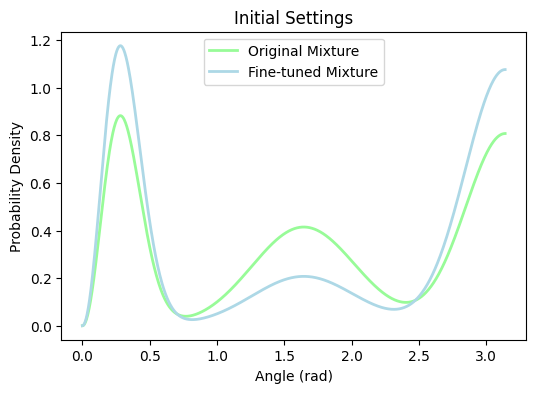
\includegraphics[width=0.6\linewidth]{figures/initial_settings.png}
    \caption{Initial settings of the three-component $\IGSO(3)$ mixture model. The original distribution (green) and the fine-tuned target distribution (blue) are shown by the marginal PDFs of the rotation angle.}
    \label{fig:initial_settings}
\end{figure}

\begin{figure}[!ht]
    \centering
    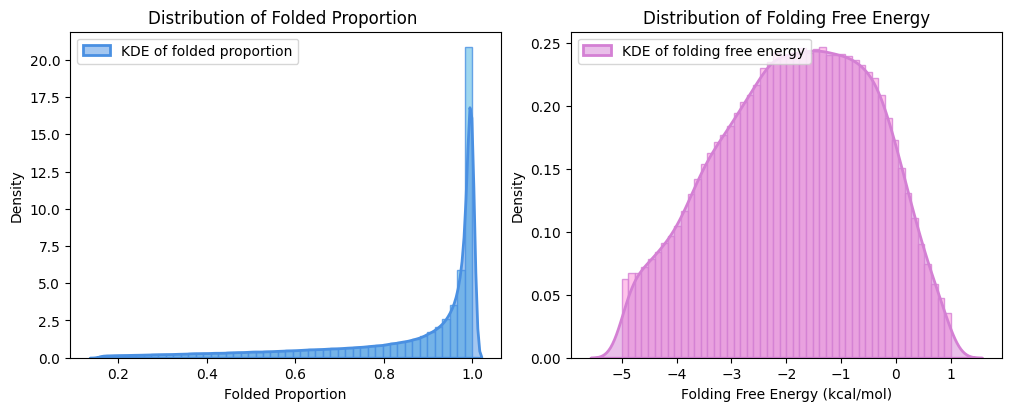
\includegraphics[width=\linewidth]{figures/data_distribution.png}
    \caption{Distribution of folded proportion and folding free energy for the whole MEGAScale dataset with $\Delta G \in [-5, 1]$ (kcal/mol) used for fine-tuning BioEmu. The folded proportion values are transformed from $\Delta G$ at the temperature of 298 K.}
    \label{fig:data_distribution}
\end{figure}

\newpage

\begin{figure}[!ht]
    \centering
    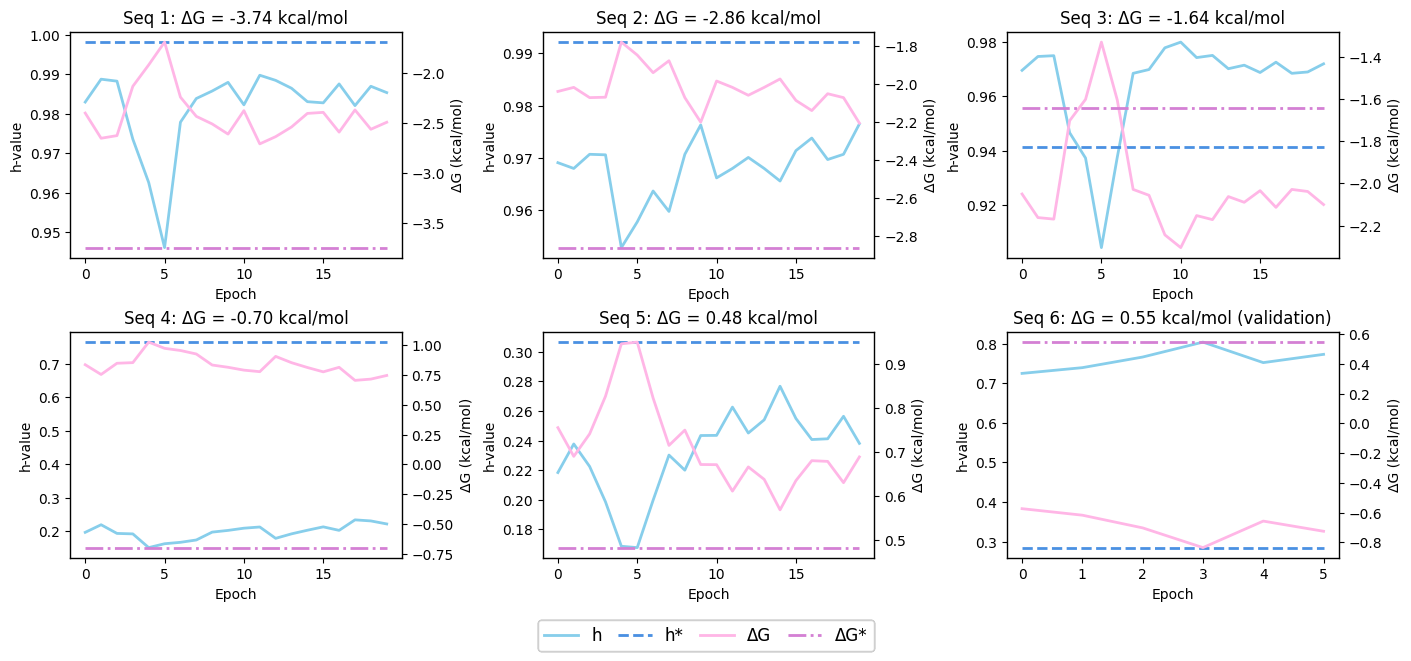
\includegraphics[width=\textwidth]{figures/finetune_h_curves_1.0e-04.png}\\
    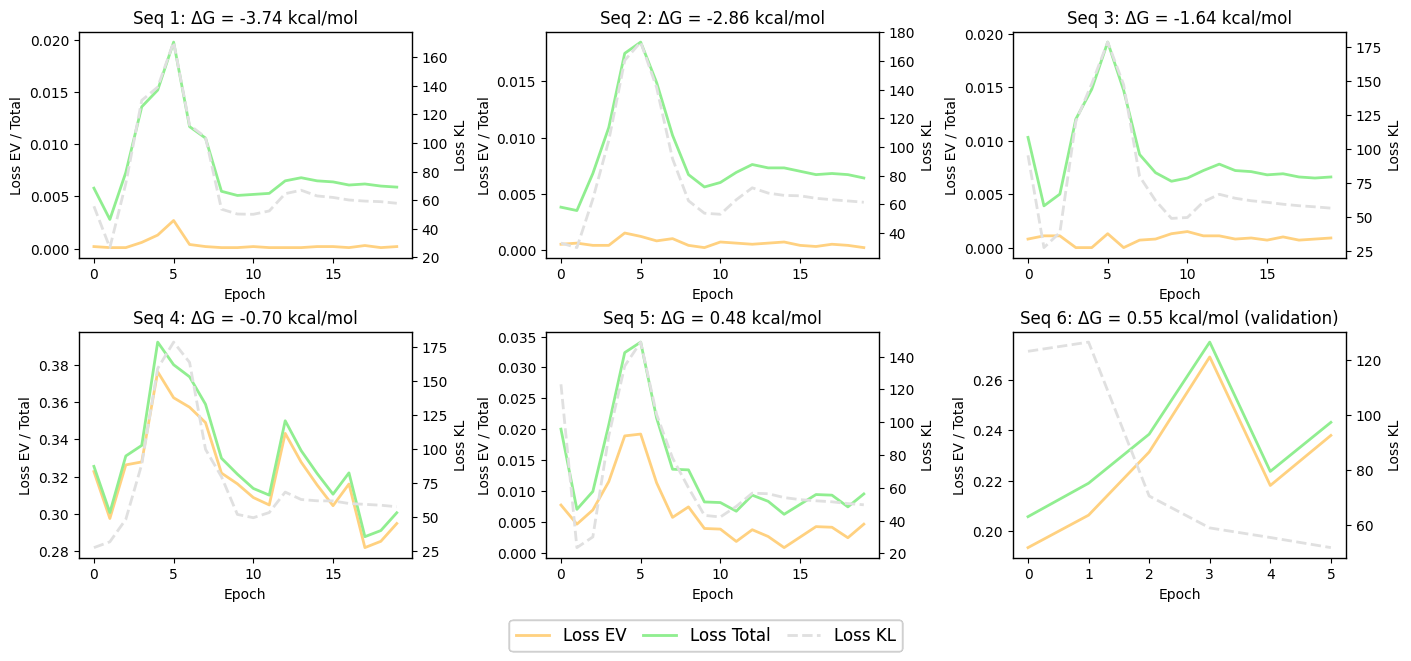
\includegraphics[width=\textwidth]{figures/finetune_loss_curves_1.0e-04.png}
    \caption{Fine-tuning curves of BioEmu with hyperparameter $\lambda=10^{-4}$.  Labelled the same as in Figure~\ref{fig:finetune_curves}.}
    \label{fig:finetune_curves_1.0e-04}
\end{figure}

\newpage

\begin{figure}[!ht]
    \centering
    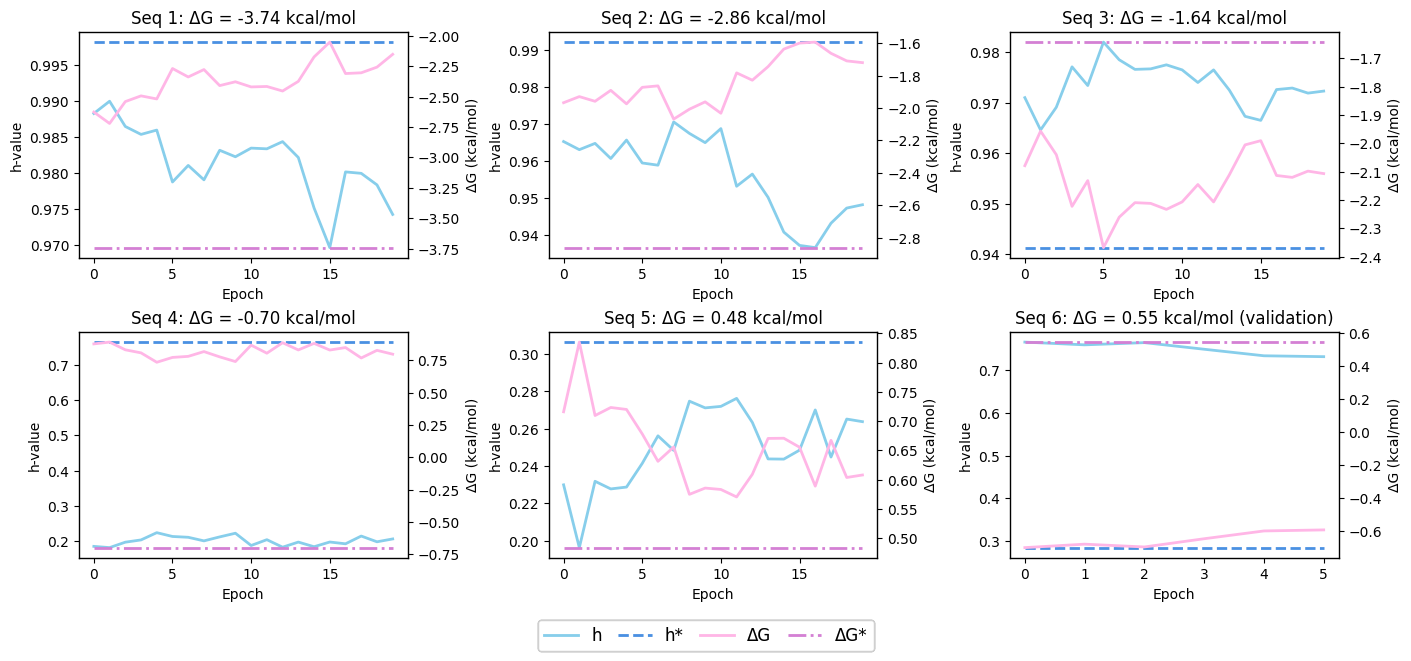
\includegraphics[width=\textwidth]{figures/finetune_h_curves_1.0e-06.png}\\
    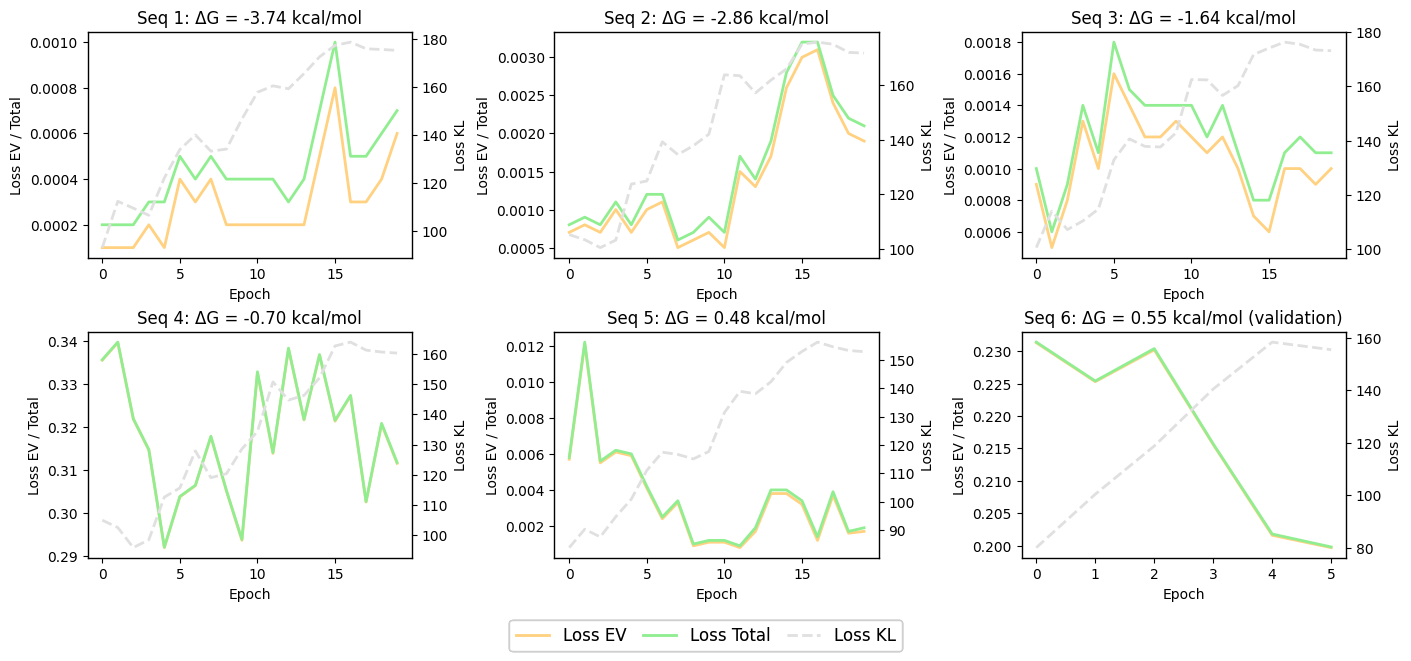
\includegraphics[width=\textwidth]{figures/finetune_loss_curves_1.0e-06.png}
    \caption{Fine-tuning curves of BioEmu with hyperparameter $\lambda=10^{-6}$. Labelled the same as in Figure~\ref{fig:finetune_curves}.}
    \label{fig:finetune_curves_1.0e-06}
\end{figure}

\newpage

\begin{figure}[!ht]
    \centering
    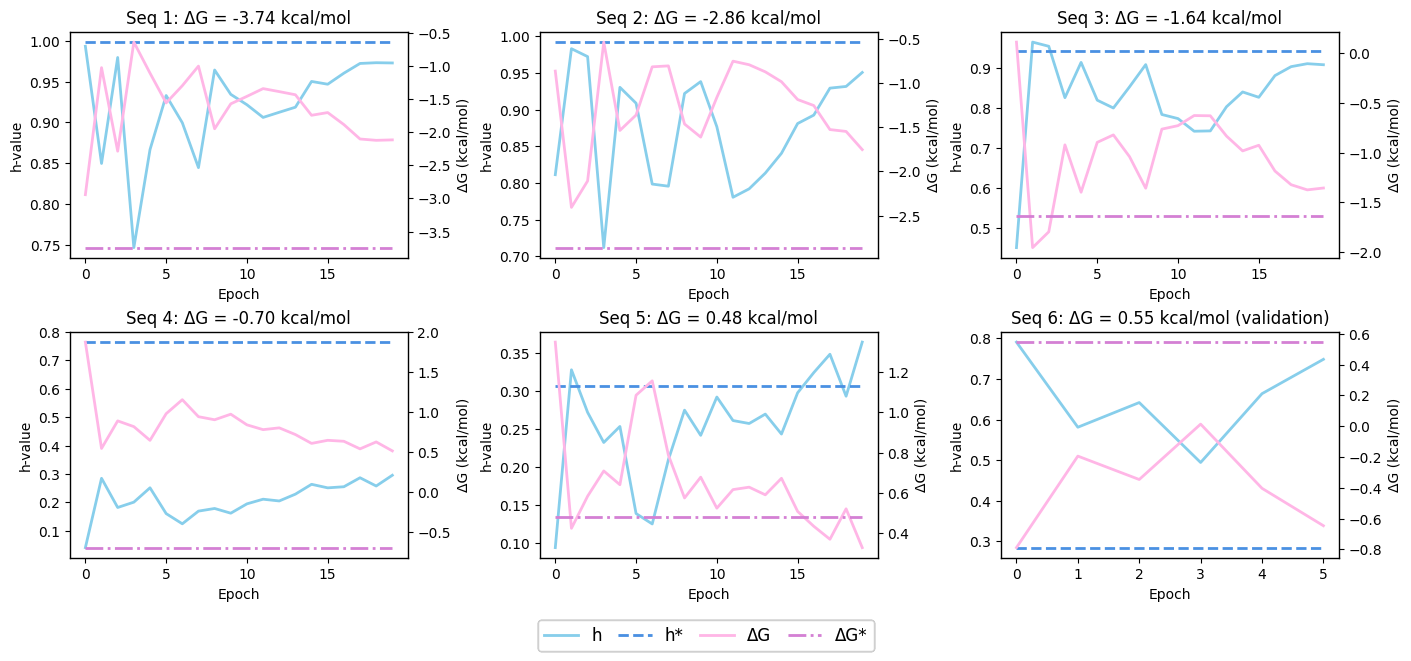
\includegraphics[width=\textwidth]{figures/finetune_h_curves_medium.png}\\
    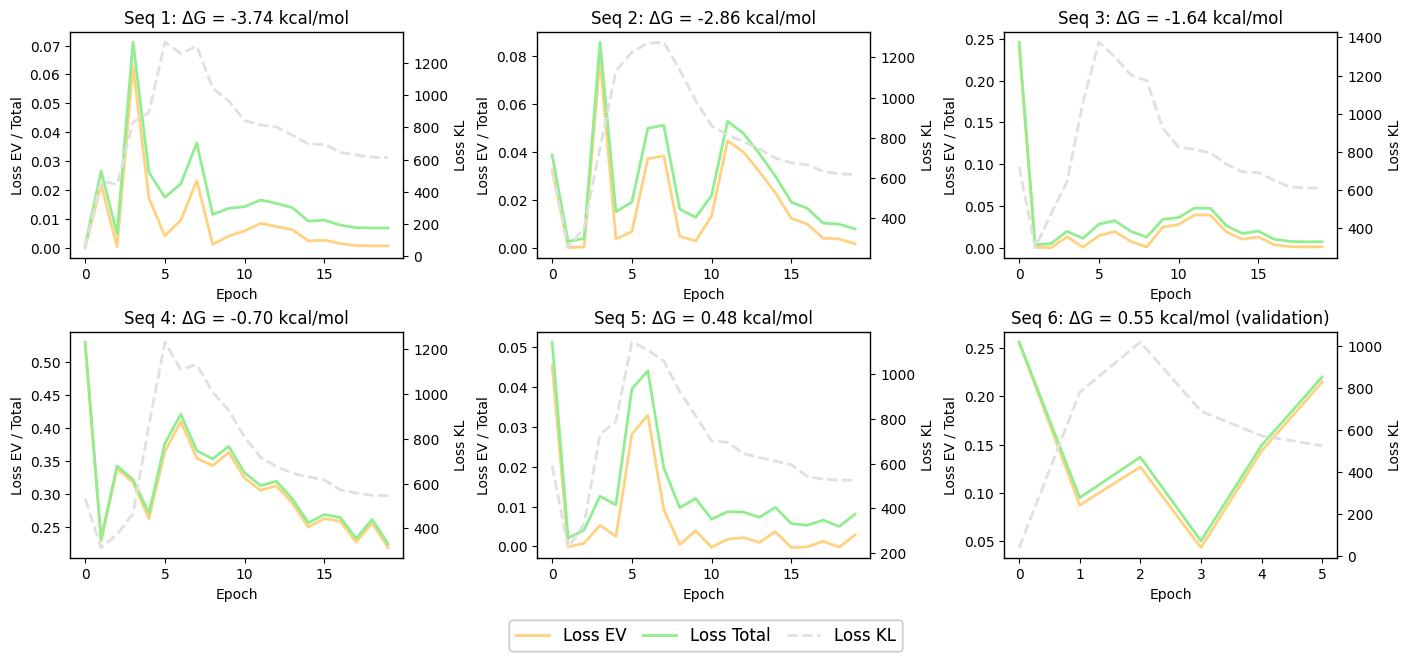
\includegraphics[width=\textwidth]{figures/finetune_loss_curves_medium.png}
    \caption{Fine-tuning curves of BioEmu with a medium size of the controller model. Labelled the same as in Figure~\ref{fig:finetune_curves}.}
    \label{fig:finetune_curves_medium}
\end{figure}

\newpage

\subsection{Supplementary tables}

\begin{table}[!ht]
\centering
\caption{Hyperparameters for Euler-Maruyama predictor}
\label{tab:euler_maruyama_finetune_hyperparameters}
\begin{tabular}{ll}
\toprule
Parameter (key) & Value \\
\midrule
Number of steps (\texttt{num\_steps}) & 200 \\
Maximum time (\texttt{max\_t}) & 0.99 \\
Minimum time (\texttt{min\_t}) & 0.001 \\
\bottomrule
\end{tabular}
\end{table}

\begin{table}[!ht]
\centering
\caption{Hyperparameters for fine-tuning BioEmu (default)}
\label{tab:finetune_hyperparameters}
\begin{tabular}{ll}
\toprule
Parameter (key) & Value \\
\midrule
Data batch size (\texttt{data\_batch\_size}) & 1 \\
Shuffle data (\texttt{shuffle}) & \texttt{True} \\
Number of workers (\texttt{num\_workers}) & 0 \\
Regularization weight (\texttt{lambda\_}) & $1\times10^{-5}$ \\
Convergence tolerance (\texttt{tol}) & $1\times10^{-7}$ \\
Batch size (\texttt{batch\_size}) & 1024 \\
Micro-batch size (\texttt{micro\_batch\_size}) & 4 \\
Number of epochs (\texttt{num\_epochs}) & 20 \\
Save interval (epochs) (\texttt{save\_every\_n\_epochs}) & 2 \\
Validation interval (epochs) (\texttt{val\_every\_n\_epochs}) & 4 \\
Learning rate (\texttt{lr}) & 5.0$\times10^{-4}$ \\
Adam betas (\texttt{betas}) & (0.9, 0.999) \\
Weight decay (\texttt{weight\_decay}) & 0.0 \\
Minimum learning rate (\texttt{eta\_min}) & $1\times10^{-5}$ \\
\bottomrule
\end{tabular}
\end{table}

\begin{table}[!ht]
\centering
\caption{Hyperparameters for folding stability estimation}
\label{tab:folding_stability_hyperparameters}
\begin{tabular}{ll}
\toprule
Parameter (key) & Value \\
\midrule
Temperature (K) (\texttt{temperature}) & 298.0 \\
Scaling constant $k$ (\texttt{k}) & -24.0 \\
Distance cutoff $d_{0}$ (nm) (\texttt{d\_0}) & 0.4 \\
Convergence tolerance (\texttt{tol}) & $1\times10^{-7}$ \\
\bottomrule
\end{tabular}
\end{table}

\begin{table}[!ht]
\centering
\caption{Hyperparameters for fine-tuned model size (default)}
\label{tab:finetune_model_size_hyperparameters}
\begin{tabular}{ll}
\toprule
Parameter (key) & Value \\
\midrule
Hidden dimension (\texttt{dim\_hidden}) & 256 \\
Model dimension (\texttt{dim\_model}) & 64 \\
Pair dimension (\texttt{dim\_pair}) & 32 \\
Single-rep dimension (\texttt{dim\_single\_rep}) & 16 \\
Dropout rate (\texttt{dropout}) & 0.1 \\
Max relative distance (\texttt{max\_distance\_relative}) & 128 \\
Number of buckets (\texttt{num\_buckets}) & 64 \\
Number of heads (\texttt{num\_heads}) & 4 \\
Number of layers (\texttt{num\_layers}) & 2 \\
\bottomrule
\end{tabular}
\end{table}

\newpage

\begin{table}[!ht]
\centering
\caption{Hyperparameters for fine-tuning BioEmu (medium)}
\label{tab:finetune_medium_hyperparameters}
\begin{tabular}{ll}
\toprule
Parameter (key) & Value \\
\midrule
Data batch size (\texttt{data\_batch\_size}) & 1 \\
Shuffle data (\texttt{shuffle}) & \texttt{True} \\
Number of workers (\texttt{num\_workers}) & 0 \\
Regularization weight (\texttt{lambda\_}) & $1\times10^{-5}$ \\
Convergence tolerance (\texttt{tol}) & $1\times10^{-7}$ \\
Batch size (\texttt{batch\_size}) & 256 \\
Micro-batch size (\texttt{micro\_batch\_size}) & 4 \\
Number of epochs (\texttt{num\_epochs}) & 20 \\
Save interval (epochs) (\texttt{save\_every\_n\_epochs}) & 2 \\
Validation interval (epochs) (\texttt{val\_every\_n\_epochs}) & 4 \\
Learning rate (\texttt{lr}) & 5.0$\times10^{-4}$ \\
Adam betas (\texttt{betas}) & (0.9, 0.999) \\
Weight decay (\texttt{weight\_decay}) & 0.0 \\
Minimum learning rate (\texttt{eta\_min}) & $1\times10^{-5}$ \\
\bottomrule
\end{tabular}
\end{table}

\begin{table}[!ht]
\centering
\caption{Hyperparameters for fine-tuned model size (medium)}
\label{tab:finetune_model_size_medium_hyperparameters}
\begin{tabular}{ll}
\toprule
Parameter (key) & Value \\
\midrule
Hidden dimension (\texttt{dim\_hidden}) & 512 \\
Model dimension (\texttt{dim\_model}) & 256 \\
Pair dimension (\texttt{dim\_pair}) & 128 \\
Single-rep dimension (\texttt{dim\_single\_rep}) & 32 \\
Dropout rate (\texttt{dropout}) & 0.1 \\
Max relative distance (\texttt{max\_distance\_relative}) & 128 \\
Number of buckets (\texttt{num\_buckets}) & 64 \\
Number of heads (\texttt{num\_heads}) & 8 \\
Number of layers (\texttt{num\_layers}) & 4 \\
\bottomrule
\end{tabular}
\end{table}

\begin{table}[!ht]
\centering
\caption{Folded proportion and experimental stability ($\Delta G_{\mathrm{exp}}$) of the 5 sequences for fine-tuning}
\label{tab:protein_summary}
\begin{tabular}{clcccc}
\toprule
Sequence ID & PDB name & $p_{\textrm{folded}}$ & $\Delta G_{\textrm{exp}}$ (kcal/mol) & CI$_{95,\textrm{low}}$ & CI$_{95,\textrm{high}}$ \\
\midrule
Seq 1 & \texttt{XX|run10\_1081\_0004.pdb\_K15I} & 0.998 & -3.726 & -3.803 & -3.653 \\
Seq 2 & \texttt{r4\_412\_TrROS\_Hall.pdb\_N12S} & 0.992 & -2.866 & -2.992 & -2.784\\
Seq 3 & \texttt{XX|run1\_0254\_0003.pdb\_L25N}   & 0.941 & -1.644 & -1.680 & -1.607 \\
Seq 4 & \texttt{2L2D.pdb\_W31I}                  & 0.764 & -0.697 & -0.796 & -0.591 \\
Seq 5 & \texttt{6OBK.pdb\_Y35P}                  & 0.307 &  0.483 & 0.375 & 0.550 \\
\bottomrule
\end{tabular}
\end{table}


\begin{table}[!ht]
\centering
\caption{Initial settings and fine-tuned target of the synthetic $\IGSO(3)$ mixture}
\label{tab:igso3_mixture_settings}
\begin{tabular}{cccccc}
\toprule
Component & Rotation axis (unit vector) & Rotation angle (rad) & $\sigma$ & Weight & Fine-tuned weight \\
\midrule
1 & N/A (identity)      & $0$               & $0.2$ & $0.3$ & $0.4$ \\
2 & $(0,\,1,\,0)$       & $\frac{\pi}{2}$  & $0.4$ & $0.4$ & $0.2$ \\
3 & $(0,\,0,\,1)$       & $\pi$             & $0.3$ & $0.3$ & $0.4$ \\
\bottomrule
\end{tabular}
\end{table}


%%%%%%%%%%%%%%%%%%%%%%%%%%%%%%%%%%%%%%%%%%%%%%%%%%%%%%%%%%%%%%%%%%%%%%%%%%%%%%%
%%%%%%%%%%%%%%%%%%%%%%%%%%%%%%%%%%%%%%%%%%%%%%%%%%%%%%%%%%%%%%%%%%%%%%%%%%%%%%%


\end{document}
